%Version 3.1 December 2024
% See section 11 of the User Manual for version history
%
%%%%%%%%%%%%%%%%%%%%%%%%%%%%%%%%%%%%%%%%%%%%%%%%%%%%%%%%%%%%%%%%%%%%%%
%%                                                                 %%
%% Please do not use \input{...} to include other tex files.       %%
%% Submit your LaTeX manuscript as one .tex document.              %%
%%                                                                 %%
%% All additional figures and files should be attached             %%
%% separately and not embedded in the \TeX\ document itself.       %%
%%                                                                 %%
%%%%%%%%%%%%%%%%%%%%%%%%%%%%%%%%%%%%%%%%%%%%%%%%%%%%%%%%%%%%%%%%%%%%%

%%\documentclass[referee,sn-basic]{sn-jnl}% referee option is meant for double line spacing

%%=======================================================%%
%% to print line numbers in the margin use lineno option %%
%%=======================================================%%

%%\documentclass[lineno,pdflatex,sn-basic]{sn-jnl}% Basic Springer Nature Reference Style/Chemistry Reference Style

%%=========================================================================================%%
%% the documentclass is set to pdflatex as default. You can delete it if not appropriate.  %%
%%=========================================================================================%%

%%\documentclass[sn-basic]{sn-jnl}% Basic Springer Nature Reference Style/Chemistry Reference Style

%% The available reference styles support both named-date and numbered citations.
%%\documentclass[pdflatex,sn-nature]{sn-jnl}% Style for submissions to Nature Portfolio journals
%%\documentclass[pdflatex,sn-basic]{sn-jnl}% Basic Springer Nature Reference Style/Chemistry Reference Style
\documentclass[pdflatex,sn-mathphys-num]{sn-jnl}% Math and Physical Sciences Numbered Reference Style
%%\documentclass[pdflatex,sn-mathphys-ay]{sn-jnl}% Math and Physical Sciences Author Year Reference Style
%%\documentclass[pdflatex,sn-aps]{sn-jnl}% American Physical Society (APS) Reference Style
%%\documentclass[pdflatex,sn-vancouver-num]{sn-jnl}% Vancouver Numbered Reference Style
%%\documentclass[pdflatex,sn-vancouver-ay]{sn-jnl}% Vancouver Author Year Reference Style
%%\documentclass[pdflatex,sn-apa]{sn-jnl}% APA Reference Style
%%\documentclass[pdflatex,sn-chicago]{sn-jnl}% Chicago-based Humanities Reference Style

%%%% Standard Packages
%%<additional latex packages if required can be included here>
\usepackage{graphicx}%
\usepackage{multirow}%
\usepackage{amsmath,amssymb,amsfonts}%
\usepackage{amsthm}%
\usepackage{mathrsfs}%
\usepackage[title]{appendix}%
\usepackage{xcolor}%
\usepackage{textcomp}%
\usepackage{manyfoot}%
\usepackage{booktabs}%
\newcommand{\Prob}{\mathbb{P}}
\usepackage{listings}%
\usepackage{algorithm}
\usepackage{algpseudocode}
\usepackage{adjustbox}
\usepackage{makecell}
\usepackage{amssymb} % for \checkmark
\usepackage{tabularx}
\usepackage{array}
\usepackage{ragged2e}
\usepackage{microtype}
\usepackage{url}
\newenvironment{changed}{\color{blue}}{}
\newcommand{\change}[1]{{\color{blue}#1}}

%% as per the requirement new theorem styles can be included as shown below
\theoremstyle{thmstyleone}%
\newtheorem{theorem}{Theorem}%  meant for continuous numbers
%%\newtheorem{theorem}{Theorem}[section]% meant for sectionwise numbers
%% optional argument [theorem] produces theorem numbering sequence instead of independent numbers for Proposition
\newtheorem{proposition}[theorem]{Proposition}%
%%\newtheorem{proposition}{Proposition}% to get separate numbers for theorem and proposition etc.

\theoremstyle{thmstyletwo}%
\newtheorem{example}{Example}%
\newtheorem{remark}{Remark}%

\theoremstyle{thmstylethree}%
\newtheorem{definition}{Definition}%

\raggedbottom
%%\unnumbered% uncomment this for unnumbered level heads

\begin{document}

\title[CA-DTNet]{\change{CA-DTNet: A Trace-Driven Communication-Aware Digital Twin Network for Robust High-Resolution Traffic Forecasting under Heterogeneous V2X Conditions}}

\author[1,2]{\fnm{Shishir Singh} \sur{Chauhan}}\email{shishir.chauhan@jaipur.manipal.edu}

\author*[2,2]{\fnm{Satyabrata} \sur{Roy}}\email{satyabrata.roy@jaipur.manipal.edu}

\equalcont{These authors contributed equally to this work.}

\affil[1,2]{\orgdiv{Department of Computer Science and Engineering}, \orgname{Manipal University Jaipur}, \orgaddress{\street{Jaipur-Ajmer Expressway}, \city{Jaipur}, \postcode{303007}, \state{Rajasthan}, \country{INDIA}}}

%%==================================%%
%% Sample for unstructured abstract %%
%%==================================%%

\abstract{\change{Reliable high-resolution traffic forecasting is essential for connected intelligent transportation systems, where observations are delivered through heterogeneous vehicular networks. Most forecasting models assume clean, immediately available measurements, although operational inputs can be stale or incomplete. This paper proposes CA-DTNet, a communication-aware digital twin network for robust short-term traffic forecasting. One-second pNEUMA traffic states are combined with ordered CICV5G and SEE-V2X trace segments through a deterministic replay protocol. Packet loss directly produces sample-and-hold observations and increasing Age of Information (AoI), while latency, jitter, load, throughput, and radio-quality measurements condition a learned reliability gate. CA-DTNet uses a shared spatiotemporal representation for clean-state reconstruction and quantile forecasts of speed, vehicle count, and flow at 5-, 10-, and 30-second horizons. Across three seeds, the model obtains the lowest mean absolute error and weighted absolute percentage error in 24 of 27 domain--horizon--target combinations. Its reconstruction \(R^{2}\) exceeds 0.985 in both communication domains. Exact matched-window analysis yields a mean absolute cross-domain MAE shift of 0.20\% and a significant domain effect in only one of nine forecasting tasks. With 71,203 trainable parameters and approximately 0.393~ms inference latency per sample, CA-DTNet improves forecasting accuracy without relying on greater capacity than DCRNN or Graph WaveNet. The results support trace-driven, uncertainty-aware traffic digital twins while also delimiting the current evidence to one traffic source and two replay domains.}}

\keywords{Traffic forecasting,
Digital twin,
Vehicular communication,
V2X networks,
Graph attention network,
Age of information,
Probabilistic forecasting,
Intelligent transportation systems}

%%\pacs[JEL Classification]{D8, H51}

%%\pacs[MSC Classification]{35A01, 65L10, 65L12, 65L20, 65L70}

\maketitle

\section{Introduction}
\label{sec:introduction}

Reliable short term traffic forecasting is an important requirement for intelligent transportation systems because traffic management, route guidance, cooperative driving, and network assisted mobility depend on an accurate representation of the current and future road state. The forecasting problem becomes more difficult when traffic information is transferred through vehicular communication networks. Measurements that are timely and complete at the sensing point may arrive at the digital platform with delay, packet loss, irregular update intervals, or temporary channel congestion. Consequently, a forecasting model can receive an observation that is not only noisy, but also stale or partially missing.

Recent traffic forecasting methods have achieved substantial progress by representing a road network as a graph and learning its spatial and temporal dependencies. Diffusion convolutional recurrent neural networks model traffic propagation through directed graph diffusion and recurrent sequence learning \cite{li2018dcrnn}. Spatio temporal graph convolutional networks combine graph convolution with temporal convolution to learn network wide traffic patterns \cite{yu2018stgcn}. Graph WaveNet further introduces adaptive graph learning and dilated temporal convolution to capture hidden spatial relations and long temporal dependencies \cite{wu2019graphwavenet}. These approaches have established strong forecasting baselines. However, their usual formulation assumes that the input traffic sequence is directly available to the forecasting model. The communication process through which traffic observations reach the digital platform is generally not represented explicitly.

This assumption is restrictive for connected and automated transportation systems. In a vehicular network, the usefulness of an observation depends on both its measured value and its information freshness. Age of information provides a principled measure of the time elapsed since the generation of the most recently received update \cite{kaul2012aoi}. Latency, packet loss, jitter, channel occupancy, received signal strength, and signal quality can also affect the reliability of the available traffic state. A forecasting model that ignores these variables cannot distinguish between a genuine change in traffic conditions and a change caused by communication impairment.

Digital twin technology offers a suitable framework for addressing this limitation. A transportation digital twin maintains a virtual representation of the physical traffic system and updates that representation as new observations become available. Such a system should not be limited to passive data replication. It should reconstruct the most plausible current state, predict future traffic evolution, and quantify uncertainty when the received information is incomplete or delayed \cite{irfan2023transportationdt}. In vehicular environments, the twin must also account for the communication conditions that connect the physical and digital spaces \cite{khan2022federateddt}. This requirement motivates a unified formulation in which communication awareness, state reconstruction, graph based forecasting, and uncertainty estimation are learned together.

Another limitation in existing evaluations is the separation between traffic datasets and communication studies. Traffic forecasting models are commonly evaluated using clean sensor measurements, whereas vehicular communication models are often analysed without measuring their effect on downstream traffic prediction. A realistic assessment requires traffic observations and communication traces to be combined without replacing either domain with an arbitrary synthetic noise model. The pNEUMA experiment provides high resolution naturalistic vehicle trajectories collected over an urban road network \cite{barmpounakis2020pneuma}. These trajectories permit the construction of one second traffic states and graph structured road observations. When real communication traces are replayed over the same traffic windows, the resulting framework can evaluate forecasting performance under measured network conditions while preserving the underlying physical traffic process.

This study introduces the Communication Aware Digital Twin Network, referred to as CA-DTNet, for reliable high resolution traffic forecasting. The framework integrates traffic observations with communication context obtained from CICV5G and SEE V2X traces. A temporal traffic encoder and a communication encoder produce complementary latent representations. A communication aware fusion mechanism combines these representations before graph attention and temporal decoding. The model contains a reconstruction head that estimates the clean digital twin state and a probabilistic forecasting head that produces median and interval forecasts for speed, vehicle count, and flow at five, ten, and thirty second horizons. Quantile regression is used to represent predictive uncertainty without imposing a fixed parametric distribution \cite{koenker1978quantile}.

The experimental design follows a trace driven protocol. The same physical traffic windows are evaluated under clean observations, CICV5G impairment, and SEE V2X impairment. This design supports both conventional forecasting comparisons and exact matched window analysis. The latter holds the traffic state constant while changing the communication domain, thereby reducing the confounding between traffic difficulty and communication quality. The proposed model is compared with DCRNN, Graph WaveNet, and Graph GRU using three independent random seeds. Component ablations evaluate the roles of communication encoding, age of information, graph attention, reconstruction supervision, and uncertainty learning.

The verified results show that CA-DTNet obtains the lowest mean absolute error and weighted absolute percentage error in twenty four of the twenty seven evaluated domain, horizon, and target combinations. Its overall weighted absolute percentage error remains nearly unchanged across clean, CICV5G, and SEE V2X conditions. The matched analysis identifies a statistically significant communication domain effect in one of nine CA-DTNet forecasting tasks, compared with five of nine tasks for Graph GRU. The reconstruction head achieves an average coefficient of determination above 0.985 in both communication domains. The model uses 71,203 trainable parameters and requires approximately 0.393 milliseconds per sample during inference. These findings indicate that the proposed framework improves average forecasting accuracy while preserving stable behaviour across heterogeneous communication conditions.

The main contributions of this study are stated as follows.

\begin{enumerate}
    \item A trace driven communication aware digital twin formulation is developed for high resolution traffic forecasting. The formulation combines naturalistic urban traffic trajectories with measured vehicular communication traces without relying on a simulator generated channel model.

    \item A unified neural architecture is proposed for communication conditioned traffic representation, graph based spatial learning, digital twin state reconstruction, and probabilistic multi horizon forecasting.

    \item An exact matched window evaluation is introduced to isolate communication domain effects from physical traffic difficulty. Each CICV5G observation is paired with the corresponding SEE V2X observation generated from the same traffic window.

    \item A comprehensive experimental study is conducted using clean and impaired observations, three random seeds, established graph forecasting baselines, component ablations, statistical tests, reconstruction analysis, uncertainty evaluation, and computational efficiency measurements.

    \item The results provide a balanced interpretation of communication awareness. Communication variables do not reduce every point forecasting metric in isolation, but they support domain awareness, state reconstruction, uncertainty modelling, and stable operation across heterogeneous vehicular network conditions.
\end{enumerate}

The remainder of the paper is organised as follows. Section~\ref{sec:related_work} reviews graph based traffic forecasting, transportation digital twins, vehicular communication awareness, and probabilistic prediction. Section~\ref{sec:system_model} defines the traffic graph, communication context, trace replay process, and forecasting problem. Section~\ref{sec:methodology} presents the CA-DTNet architecture and training objectives. Section~\ref{sec:experimental_setup} describes the datasets, preprocessing, baselines, evaluation protocol, and metrics. Section~\ref{sec:results} reports forecasting, reconstruction, uncertainty, robustness, ablation, and efficiency results. Section~\ref{sec:discussion} discusses the findings and limitations. Section~\ref{sec:conclusion} concludes the paper.

\section{Related Work}
\label{sec:related_work}

The proposed CA-DTNet framework lies at the intersection of traffic forecasting, graph based spatial temporal learning, vehicular communication, digital twin modelling, and probabilistic prediction. These research streams have developed rapidly, but they have mostly progressed in parallel. Traffic forecasting studies usually focus on modelling spatial and temporal traffic dependencies. Vehicular communication studies usually focus on link reliability, latency, information freshness, and network quality. Digital twin studies provide a system level vision for synchronising physical and virtual systems, while probabilistic forecasting studies quantify predictive uncertainty. The central motivation of this manuscript is that a practical traffic digital twin for connected vehicular environments must combine these streams in one trace driven learning framework.

\subsection{Graph based traffic forecasting}

Road traffic is naturally structured over a graph because each road segment or sensor is influenced by neighbouring segments, upstream and downstream flow, intersection geometry, lane connectivity, and hidden functional relations. Graph neural networks are therefore widely used in traffic forecasting because they can represent such spatial dependencies more directly than independent time series models. General graph convolutional and graph attention mechanisms introduced by Kipf and Welling \cite{kipf2017gcn} and Velickovic et al. \cite{velickovic2018gat} provided the methodological basis for several traffic forecasting architectures. Surveys by Jiang and Luo \cite{jiang2022gnnsurvey} and Jin et al. \cite{jin2023stgnnsurvey} show that graph based traffic forecasting has become a dominant research direction in urban computing and intelligent transportation.

DCRNN is one of the earliest influential graph recurrent models for traffic forecasting. It models traffic diffusion over directed graphs and uses recurrent units to learn temporal evolution \cite{li2018dcrnn}. STGCN replaces recurrent computation with temporal convolution and graph convolution, which improves efficiency and captures local spatial temporal patterns \cite{yu2018stgcn}. ASTGCN extends this idea by introducing spatial and temporal attention, allowing the model to assign different importance to different road segments and time steps \cite{guo2019astgcn}. Graph WaveNet combines dilated temporal convolution with adaptive adjacency learning, enabling the discovery of latent spatial relations that are not fully represented by a predefined road graph \cite{wu2019graphwavenet}. AGCRN further learns node adaptive parameters and adaptive graph structures, reducing dependence on fixed graph assumptions \cite{bai2020agcrn}. These models establish the graph forecasting foundations on which the present work builds.

Recent graph forecasting research has also examined whether complex graph designs are always necessary. MTGNN learns directional dependencies among variables and is widely used for multivariate time series forecasting beyond traffic applications \cite{wu2020mtgnn}. StemGNN models both temporal and inter series dependencies in the spectral domain \cite{cao2021stemgnn}. STID demonstrates that simple spatial temporal identity embeddings can provide strong forecasting performance, which suggests that part of the performance gain may arise from effective representation rather than increasingly complex propagation mechanisms \cite{shao2022stid}. STEP shows that spatial temporal graph neural networks can benefit from pretraining, indicating that learned temporal representations can transfer across forecasting tasks \cite{shao2022step}. SimST argues that efficient and simplified spatial modelling can compete with heavier graph neural networks under certain conditions \cite{liu2023simst}. These studies are important for the present manuscript because CA-DTNet must not be evaluated only against weak recurrent baselines. For this reason, the experimental section compares CA-DTNet against DCRNN, Graph WaveNet, and Graph GRU.

Despite their strength, most graph based traffic forecasting models assume that traffic observations are already available to the prediction model in a reliable form. They focus on the physical traffic process but do not explicitly model the communication process through which traffic states are delivered to the digital platform. In real vehicular systems, the input sequence may be delayed, stale, incomplete, or affected by packet loss and channel congestion. This gap motivates communication aware traffic forecasting.

\subsection{Transformer based spatial temporal forecasting}

Transformer based forecasting models have become increasingly important because attention mechanisms can capture long range dependencies without the sequential bottleneck of recurrent networks. GMAN applies graph multi attention to traffic prediction and jointly models spatial and temporal dependencies through attention modules \cite{zheng2020gman}. Traffic Transformer introduces attention based dynamic spatial temporal representation learning for traffic sequence modelling \cite{yan2021traffictransformer}. PDFormer explicitly considers propagation delay and dynamic long range dependency, making it particularly relevant for traffic flow propagation across road networks \cite{jiang2023pdformer}. STAEformer shows that adaptive spatial temporal embeddings can make a comparatively simple Transformer highly competitive for traffic forecasting \cite{liu2023staeformer}. STGformer focuses on efficient graph Transformer modelling for traffic forecasting and attempts to balance accuracy with computational cost \cite{wang2024stgformer}.

\begin{changed}
Recent 2024 work further emphasizes the accuracy--scalability trade-off. STGformer combines graph structure with linearized attention for large road networks, while STGAFormer uses gated spatial--temporal attention and PatchSTG dynamically organizes large-scale spatial dependencies \cite{wang2024stgformer,li2024stgaformer,zhang2024patchstg}. These models strengthen the traffic-only forecasting frontier. They are not direct substitutes for CA-DTNet, however, because their published inputs do not contain replayed V2X quality variables or a clean-state reconstruction target. We therefore include them as state-of-the-art methodological comparators in Table~\ref{tab:related_work_summary} and explicitly avoid presenting the graph baselines as an exhaustive ranking against every Transformer architecture.
\end{changed}

These Transformer based studies demonstrate that adaptive representation learning is useful for traffic forecasting. However, their attention mechanisms are mainly designed to learn dependencies among road segments and time steps. They do not generally represent communication context such as delay, age of information, packet loss, jitter, throughput, signal strength, or signal quality. In contrast, CA-DTNet uses communication features as part of the input representation, so that the model can learn whether the received traffic state is likely to be reliable or affected by the network condition.

\subsection{Vehicular communication and information freshness}

Vehicular communication is a key enabler of connected and automated mobility. LTE V2X, NR V2X, and IEEE 802.11 based vehicular communication technologies have been studied extensively for vehicle to vehicle, vehicle to infrastructure, and vehicle to network services. Molina Masegosa and Gozalvez \cite{molinamasegosa2017ltev} discuss LTE V2X sidelink communication as an important technology for short range vehicular services. Naik et al. \cite{naik2019v2x} review the evolution from IEEE 802.11p toward IEEE 802.11bd and 5G NR V2X. Garcia et al. \cite{garcia2021nrv2x} provide a detailed tutorial on 5G NR V2X communication. 3GPP technical specifications define architectural and radio access support for V2X services in cellular systems \cite{3gpp23287,3gpp38300}. Broader 6G oriented studies argue that future vehicular systems will require ultra reliable, low latency, and context aware communication for cooperative mobility \cite{giordani2020toward6g,shafin2020artificialintelligence6g}.

In vehicular systems, the usefulness of a received message depends not only on whether the message arrives, but also on how fresh the message is. Age of information is therefore highly relevant. It measures the time elapsed since the generation of the most recently received update. Sun et al. \cite{sun2017update} show that update timing has a direct effect on data freshness. Kadota et al. \cite{kadota2018aoi} study scheduling policies for minimizing age of information in wireless broadcast networks. Talak et al. \cite{talak2020aoi} analyse information freshness in wireless networks under random service processes. Yates et al. \cite{yates2021aoi} provide a comprehensive introduction and survey of age of information. These studies show that freshness is a measurable communication property and should be considered when the downstream application relies on timely state updates.

However, the connection between vehicular communication metrics and downstream traffic forecasting is still underdeveloped. Networking studies often report communication performance in terms of latency, reliability, throughput, or age of information, but they do not usually evaluate how these metrics affect traffic prediction accuracy. Traffic forecasting studies usually report prediction metrics but do not include communication variables as part of the learning process. CA-DTNet addresses this separation by treating communication context as an input to the digital twin model. This makes it possible to evaluate not only whether a model predicts well, but also whether it remains stable when the same traffic state is observed under different measured communication conditions.

\begin{changed}
Recent vehicular-network studies make the application relevance of freshness and resource contention especially clear. Priority-aware multi-agent reinforcement learning has been used to schedule C-V2X Mode~4 resources under message-priority, density, and interference constraints \cite{shakir2025priority}. AoI-aware parameterized deep Q-networks jointly select mode, channel, and power for platoon communication \cite{shakir2026pdqn}, while a 2024 systematic review organizes RSU data exchange around deployment, management, security, datasets, and evaluation metrics \cite{shakir2024rsu}. These studies optimize or review the communication subsystem itself. CA-DTNet addresses a complementary downstream question: given measured communication conditions, how should a traffic digital twin interpret the received state, reconstruct the clean present, and forecast the future? This distinction prevents resource-allocation gains from being conflated with forecasting gains.
\end{changed}

\subsection{Transportation digital twins}

A digital twin links a physical system with a continuously updated virtual representation. Fuller et al. \cite{fuller2020digitaltwin} describe digital twins as systems enabled by sensing, data integration, modelling, and feedback. Rasheed et al. \cite{rasheed2020digitaltwin} discuss digital twin values and modelling challenges. Jones et al. \cite{jones2020characterising} provide a systematic characterisation of digital twin concepts, while VanDerHorn and Mahadevan \cite{vanderhorn2021digitaltwin} discuss generalisation and implementation issues. These studies emphasise that a digital twin must be more than a static simulation. It must remain connected to the physical process and update its internal state using available observations.

In transportation, digital twins are increasingly used as a framework for mobility monitoring, infrastructure management, traffic control, and decision support. Wang et al. \cite{wang2022mobilitydt} describe the mobility digital twin concept and discuss its architecture and future challenges. Irfan et al. \cite{irfan2023transportationdt} review transportation digital twin systems for traffic safety and mobility applications. Khan et al. \cite{khan2023federateddt} discuss digital twin based vehicular networks and highlight the role of communication, privacy, and distributed learning. Errandonea et al. \cite{errandonea2020maintenance} show that digital twin technology can support predictive maintenance by connecting state monitoring with decision support. Lu et al. \cite{lu2020digitaltwin} discuss smart manufacturing digital twins, which is useful for understanding how digital twins combine data, models, and feedback in cyber physical systems.

For traffic forecasting, the digital twin idea implies two requirements. First, the virtual state should reconstruct the present physical traffic condition as accurately as possible. Second, the twin should forecast future states and indicate its uncertainty when observations are imperfect. Existing transportation digital twin studies often emphasise architecture, simulation, or system level integration. CA-DTNet focuses on a specific learning problem within this broader vision: reconstructing a clean traffic state and forecasting future traffic under measured vehicular communication impairments.

\subsection{Probabilistic forecasting and uncertainty modelling}

Point forecasts are useful, but they are incomplete for safety critical and communication dependent transportation systems. A model can have a low average error and still be unreliable under rare events, channel impairment, or rapidly changing traffic states. Probabilistic forecasting addresses this limitation by estimating a distribution or interval of plausible future outcomes. Quantile regression provides a classical foundation for estimating conditional quantiles without assuming a fixed error distribution \cite{koenker1978quantile}. Gneiting and Raftery \cite{gneiting2007scoring} explain that probabilistic forecasts should be assessed using proper scoring rules and must balance calibration with sharpness.

Deep probabilistic time series models have developed rapidly. DeepAR uses autoregressive recurrent networks to produce probabilistic forecasts across related time series \cite{salinas2020deepar}. The Temporal Fusion Transformer combines attention, gating, static covariate encoders, and quantile outputs for interpretable multi horizon forecasting \cite{lim2021tft}. Wen et al. \cite{wen2017mqrf} introduce a multi horizon quantile recurrent forecaster that directly estimates multiple future quantiles. Kuleshov et al. \cite{kuleshov2018calibration} show that deep uncertainty estimates may require calibration. Romano et al. \cite{romano2019cqr} propose conformalized quantile regression for distribution free interval calibration. Angelopoulos and Bates \cite{angelopoulos2023conformal} provide a broad introduction to conformal prediction and uncertainty quantification.

The uncertainty component of CA-DTNet follows this line of work but applies it to a communication aware traffic digital twin setting. The model predicts multiple quantiles for speed, vehicle count, and flow, and the evaluation reports both prediction interval coverage probability and prediction interval normalized average width. This is important because a model can increase coverage by producing very wide intervals. CA-DTNet therefore evaluates whether the uncertainty interval is both reliable and reasonably sharp.

\subsection{Synthesis of literature and positioning of CA-DTNet}

Table~\ref{tab:related_work_summary} summarises representative studies and compares them with the requirements of the present manuscript. The comparison shows that existing methods usually address only part of the problem. Graph and Transformer forecasting models provide strong spatial temporal prediction, but they usually do not use communication traces. Vehicular communication studies measure network quality, but they do not usually evaluate its effect on downstream forecasting. Digital twin studies provide a system concept, but they often do not present a trace driven learning model that jointly reconstructs and forecasts traffic states. Probabilistic forecasting studies quantify uncertainty, but they rarely connect uncertainty to measured communication impairment.

\begin{table}[!htbp]
\caption{Positioning of representative literature with respect to the requirements of CA-DTNet.}
\label{tab:related_work_summary}
\centering
\footnotesize
\renewcommand{\arraystretch}{1.18}
\setlength{\tabcolsep}{3pt}

\begin{tabularx}{\linewidth}{
>{\RaggedRight\arraybackslash}p{2.5cm}
>{\RaggedRight\arraybackslash}X
>{\Centering\arraybackslash}p{1.0cm}
>{\Centering\arraybackslash}p{1.0cm}
>{\Centering\arraybackslash}p{1.0cm}
>{\Centering\arraybackslash}p{1.0cm}
}
\toprule
\textbf{Study Category} &
\textbf{Main Modelling Focus} &
\textbf{Road Graph} &
\textbf{Comm. Context} &
\textbf{Twin State} &
\textbf{Prob. Forecast} \\
\midrule

Graph recurrent forecasting
\cite{li2018dcrnn,bai2020agcrn}
&
Learns temporal evolution and graph-based traffic diffusion.
&
Yes & No & No & No \\

Graph convolution and attention forecasting
\cite{yu2018stgcn,guo2019astgcn,wu2019graphwavenet}
&
Captures spatial and temporal traffic dependencies using graph convolution and attention.
&
Yes & No & No & No \\

Adaptive graph and efficient baselines
\cite{wu2020mtgnn,cao2021stemgnn,shao2022stid,shao2022step,liu2023simst}
&
Learns hidden graph dependencies, pretrained representations, and efficient spatio-temporal features.
&
Yes & No & No & No \\

Transformer-based traffic forecasting
  \cite{zheng2020gman,yan2021traffictransformer,jiang2023pdformer,liu2023staeformer,wang2024stgformer,li2024stgaformer,zhang2024patchstg}
&
Uses attention mechanisms to capture long-range spatial and temporal dependencies.
&
Yes &
No &
No &
Partial \\

Vehicular communication and V2X studies
  \cite{molinamasegosa2017ltev,naik2019v2x,garcia2021nrv2x,shakir2025priority,shakir2026pdqn,shakir2024rsu}
&
Studies communication standards, latency, reliability, and network services.
&
No &
Yes &
No &
No \\

Age of Information studies
\cite{sun2017update,kadota2018aoi,talak2020aoi,yates2021aoi}
&
Measures freshness and timeliness of communication updates.
&
No &
Yes &
No &
No \\

Digital twin studies
\cite{fuller2020digitaltwin,rasheed2020digitaltwin,jones2020characterising,vanderhorn2021digitaltwin,wang2022mobilitydt,irfan2023transportationdt,khan2023federateddt}
&
Models cyber--physical synchronization and digital twin representations.
&
Partial &
Partial &
Yes &
Partial \\

Probabilistic forecasting studies
\cite{koenker1978quantile,gneiting2007scoring,salinas2020deepar,lim2021tft,romano2019cqr,angelopoulos2023conformal}
&
Estimates predictive uncertainty using quantiles and calibrated prediction intervals.
&
No &
No &
No &
Yes \\

\textbf{CA-DTNet}
&
\textbf{Joint communication-aware traffic representation, digital twin reconstruction, graph forecasting, and uncertainty estimation.}
&
\textbf{Yes} &
\textbf{Yes} &
\textbf{Yes} &
\textbf{Yes} \\

\bottomrule
\end{tabularx}
\end{table}

The comparison in Table~\ref{tab:related_work_summary} clarifies the research gap. Existing traffic forecasting methods are strong in spatial temporal modelling, but their input formulation is usually communication agnostic. Existing vehicular communication studies are strong in network quality analysis, but they rarely measure how network variation changes forecasting performance. Existing transportation digital twin studies define the system concept, but many do not provide a concrete end to end neural model that reconstructs a clean traffic state from impaired observations and forecasts future traffic with uncertainty. Existing probabilistic forecasting methods estimate intervals, but the uncertainty is not usually conditioned on measured vehicular communication quality.

CA-DTNet is designed to fill this gap. It combines real traffic trajectories and real vehicular communication traces through a trace driven replay protocol. It learns traffic and communication representations jointly, reconstructs the clean digital twin state, produces probabilistic multi horizon forecasts, and evaluates matched communication domain robustness by pairing CICV5G and SEE V2X observations generated from the same traffic windows. This positioning is directly aligned with the manuscript objective stated in Section~\ref{sec:introduction}: to develop a communication aware digital twin for reliable high resolution traffic forecasting under heterogeneous vehicular network conditions.

\section{System Model and Problem Formulation}
\label{sec:system_model}

This section defines the traffic graph, communication context, trace driven observation process, digital twin state reconstruction task, and probabilistic forecasting objective used in this study. The formulation is designed to remain consistent with the motivation and literature gap discussed in Sections~\ref{sec:introduction} and~\ref{sec:related_work}. The central idea is that a traffic forecasting model should not only learn from traffic history, but should also account for the communication condition through which the traffic state is delivered to the digital platform.

\subsection{Notation}

Let the urban road environment be represented as a graph
\begin{equation}
    \mathcal{G} = \left(\mathcal{V}, \mathcal{E}, \mathbf{A}\right),
\end{equation}
where \(\mathcal{V}\) denotes the set of traffic nodes, \(\mathcal{E}\) denotes the set of edges that represent spatial relations among nodes, and \(\mathbf{A}\in\mathbb{R}^{N\times N}\) denotes the adjacency matrix. Here, \(N = |\mathcal{V}|\) is the number of nodes. A node can represent a road segment, lane group, or spatially aggregated traffic unit, depending on the resolution of the processed pNEUMA trajectory data.

At each discrete time instant \(t\), the clean traffic state is defined as
\begin{equation}
    \mathbf{X}_{t} \in \mathbb{R}^{N\times F},
\end{equation}
where \(F\) is the number of traffic state variables. In this manuscript, the primary traffic targets are speed, vehicle count, and flow. The historical traffic input over a look back window of length \(T\) is written as
\begin{equation}
    \mathbf{X}_{t-T+1:t} =
    \left[
    \mathbf{X}_{t-T+1},
    \mathbf{X}_{t-T+2},
    \ldots,
    \mathbf{X}_{t}
    \right].
\end{equation}

The communication condition associated with a traffic observation is represented as
\begin{equation}
    \mathbf{C}_{t} \in \mathbb{R}^{N\times M},
\end{equation}
where \(M\) is the number of communication related variables. The communication vector includes latency, age of information, packet loss, jitter, channel busy ratio, throughput, received signal reference power, and signal to interference plus noise ratio when available from the corresponding trace. The communication input over the same look back window is denoted by
\begin{equation}
    \mathbf{C}_{t-T+1:t} =
    \left[
    \mathbf{C}_{t-T+1},
    \mathbf{C}_{t-T+2},
    \ldots,
    \mathbf{C}_{t}
    \right].
\end{equation}

The main notation used in this study is summarised in Table~\ref{tab:notation_system_model}.

\begin{table}[t]
\centering
\caption{Main notation used in the system model.}
\label{tab:notation_system_model}
\small
\begin{tabular}{p{2.2cm} p{5.8cm}}
\hline
Symbol & Description \\
\hline
\(\mathcal{G}\) & Traffic graph used to represent the road network structure \\
\(\mathcal{V}\) & Set of traffic nodes \\
\(\mathcal{E}\) & Set of graph edges \\
\(\mathbf{A}\) & Adjacency matrix of the traffic graph \\
\(N\) & Number of traffic nodes \\
\(F\) & Number of traffic state variables \\
\(M\) & Number of communication state variables \\
\(\mathbf{X}_{t}\) & Clean traffic state at time \(t\) \\
\(\widetilde{\mathbf{X}}_{t}\) & Communication impaired traffic observation at time \(t\) \\
\(\widehat{\mathbf{X}}_{t}\) & Reconstructed digital twin traffic state at time \(t\) \\
\(\mathbf{C}_{t}\) & Communication context at time \(t\) \\
\(T\) & Length of the historical look back window \\
\(\tau\) & Forecasting horizon \\
\(\mathcal{H}\) & Set of forecasting horizons \\
\(\widehat{\mathbf{Y}}_{t+\tau}\) & Predicted traffic target at horizon \(\tau\) \\
\(\widehat{\mathbf{Y}}^{q}_{t+\tau}\) & Predicted quantile at level \(q\) and horizon \(\tau\) \\
\hline
\end{tabular}
\end{table}

\subsection{Traffic graph representation}

The traffic graph is constructed from the processed pNEUMA trajectory data. Each node corresponds to a spatial traffic unit for which the traffic variables can be aggregated at one second resolution. The graph adjacency matrix represents the spatial relation among traffic units. This relation can be obtained from road connectivity, spatial proximity, or the processed topology of the observed road environment.

For each node \(i\in\mathcal{V}\), the traffic feature vector at time \(t\) is expressed as
\begin{equation}
    \mathbf{x}_{i,t}
    =
    \left[
    v_{i,t},
    n_{i,t},
    f_{i,t}
    \right],
\end{equation}
where \(v_{i,t}\) is the mean speed, \(n_{i,t}\) is the vehicle count, and \(f_{i,t}\) is the flow proxy. The full traffic state matrix is therefore
\begin{equation}
    \mathbf{X}_{t}
    =
    \left[
    \mathbf{x}_{1,t},
    \mathbf{x}_{2,t},
    \ldots,
    \mathbf{x}_{N,t}
    \right]^{\top}.
\end{equation}

The purpose of the graph representation is to allow the forecasting model to learn how traffic conditions at one node influence traffic states at related nodes. This is necessary because congestion, vehicle queues, and speed changes propagate through the road network rather than remaining isolated at a single location.

\subsection{Communication context representation}

In a connected vehicular environment, the traffic state is not directly available to the digital platform. It is observed through a communication channel that may introduce delay, information staleness, packet loss, and other quality variations. Therefore, the received traffic observation may differ from the clean physical state. We denote the communication impaired traffic observation by
\begin{equation}
    \widetilde{\mathbf{X}}_{t}.
\end{equation}

The communication context at time \(t\) is represented as
\begin{equation}
    \mathbf{c}_{i,t}
    =
    \left[
    d_{i,t},
    a_{i,t},
    p_{i,t},
    j_{i,t},
    b_{i,t},
    r_{i,t},
    s_{i,t},
    z_{i,t}
    \right],
\end{equation}
where \(d_{i,t}\) denotes latency, \(a_{i,t}\) denotes age of information, \(p_{i,t}\) denotes packet loss, \(j_{i,t}\) denotes jitter, \(b_{i,t}\) denotes channel busy ratio, \(r_{i,t}\) denotes throughput, \(s_{i,t}\) denotes received signal reference power, and \(z_{i,t}\) denotes signal to interference plus noise ratio. The complete communication context matrix is written as
\begin{equation}
    \mathbf{C}_{t}
    =
    \left[
    \mathbf{c}_{1,t},
    \mathbf{c}_{2,t},
    \ldots,
    \mathbf{c}_{N,t}
    \right]^{\top}.
\end{equation}

The communication variables are not treated as prediction targets. Instead, they are used as contextual information that helps the model interpret the reliability and freshness of the received traffic state.

\subsection{Trace driven observation process}

\begin{changed}
The clean traffic states and communication traces were recorded in different experiments and therefore do not share a physical clock or geographic coordinate frame. The replay is consequently an index-aligned stress-replay procedure, not a claim that a CICV5G or SEE-V2X radio measurement was collected at a particular pNEUMA road cell. This distinction is important for interpreting external validity.

Traffic trajectories are aggregated into one-second bins and sorted by node identifier and time. Within each communication file, samples are sorted by their recorded \texttt{sample\_index}; thus, delay, loss, jitter, load, throughput, and radio-quality co-variation is preserved in its measured order. Let trace \(r\) contain \(L_r\) ordered samples. For road node \(i\), a trace is assigned deterministically by cycling through sorted trace identifiers, and a contiguous start offset \(o_i\) is drawn using the fixed replay seed. The communication row paired with the \(k\)-th traffic bin is
\begin{equation}
    \kappa(i,k)=1+\bigl((o_i+k-2)\bmod L_{r(i)}\bigr).
\end{equation}
When a trace is longer than the node sequence, a single non-wrapping contiguous segment is selected; when it is shorter, the ordered trace is repeated. This rule preserves local temporal structure and prevents per-sample cherry-picking of favorable network conditions.

Packet delivery is the only communication variable that directly replaces a traffic value. If the selected row reports loss probability \(p_{i,k}\), a seeded Bernoulli draw gives \(R_{i,k}\sim\mathrm{Bernoulli}(1-p_{i,k})\). The received state follows a sample-and-hold rule,
\begin{equation}
\widetilde{\mathbf{x}}_{i,k}=
\begin{cases}
\mathbf{x}_{i,k}, & R_{i,k}=1,\\
\widetilde{\mathbf{x}}_{i,k-1}, & R_{i,k}=0,
\end{cases}
\end{equation}
so a lost update produces staleness rather than artificial additive noise. With measured latency \(d_{i,k}\) in milliseconds and traffic-bin duration \(\Delta t=1\)~s, AoI evolves as
\begin{equation}
a_{i,k}=
\begin{cases}
\min(d_{i,k}/1000,5), & R_{i,k}=1,\\
a_{i,k-1}+\Delta t, & R_{i,k}=0.
\end{cases}
\end{equation}
The 5-s cap limits isolated extreme timestamps. Jitter, channel busy ratio, throughput, RSRP, SINR, and the uncapped standardized latency/loss measurements are supplied as context to the reliability gate; they do not independently add noise to speed, count, or flow. Stating this separation makes clear which metrics generate the impaired observation and which help the network interpret its reliability.

For every physical traffic window, the clean target and window index are retained while CICV5G and SEE-V2X are replayed separately, producing
\begin{equation}
\left(\mathbf{X}_{t-T+1:t},
\widetilde{\mathbf{X}}^{cic}_{t-T+1:t},
\widetilde{\mathbf{X}}^{see}_{t-T+1:t}\right).
\end{equation}
Assignment and offsets depend only on sorted identifiers and the fixed seed, never on future targets or forecasting errors. All models receive the same realized impaired arrays, and scaling parameters are estimated from the chronological training partition only. These controls avoid outcome-dependent traffic--communication pairing. The matched-window analysis then changes the communication domain while holding the physical traffic history fixed.
\end{changed}

\subsection{Digital twin state reconstruction}

A communication aware traffic digital twin should estimate the clean traffic state even when the received observation is impaired. Therefore, CA-DTNet includes a reconstruction task. Given the impaired traffic history and communication context, the model estimates the clean traffic state:
\begin{equation}
    \widehat{\mathbf{X}}_{t}
    =
    f_{rec}
    \left(
    \widetilde{\mathbf{X}}_{t-T+1:t},
    \mathbf{C}_{t-T+1:t},
    \mathbf{A}
    \right),
\end{equation}
where \(f_{rec}(\cdot)\) denotes the digital twin reconstruction function. The reconstruction objective is defined as
\begin{equation}
    \mathcal{L}_{rec}
    =
    \frac{1}{N F}
    \sum_{i=1}^{N}
    \sum_{k=1}^{F}
    \left|
    X_{i,t}^{k}
    -
    \widehat{X}_{i,t}^{k}
    \right|.
\end{equation}

This reconstruction objective encourages the model to learn a latent representation that is not only useful for future forecasting, but also consistent with the current physical traffic state. This is important for digital twin operation because the virtual representation must remain aligned with the physical system.

\subsection{Multi horizon traffic forecasting}

The forecasting task predicts future traffic states for multiple horizons. Let
\begin{equation}
    \mathcal{H} = \left\{5, 10, 30\right\}
\end{equation}
denote the set of forecasting horizons in seconds. For each horizon \(\tau \in \mathcal{H}\), the model predicts the future target
\begin{equation}
    \mathbf{Y}_{t+\tau}
    =
    \left[
    \mathbf{y}_{1,t+\tau},
    \mathbf{y}_{2,t+\tau},
    \ldots,
    \mathbf{y}_{N,t+\tau}
    \right]^{\top},
\end{equation}
where each target vector contains speed, vehicle count, and flow related information.

The deterministic median prediction is represented as
\begin{equation}
    \widehat{\mathbf{Y}}_{t+\tau}^{0.50}
    =
    f_{\tau}
    \left(
    \widetilde{\mathbf{X}}_{t-T+1:t},
    \mathbf{C}_{t-T+1:t},
    \mathbf{A}
    \right).
\end{equation}

The model is trained for all horizons jointly so that the learned representation supports short and relatively longer range traffic prediction. This is consistent with the practical requirements of traffic management, where decisions may depend on different prediction lead times.

\subsection{Probabilistic forecasting formulation}

Since communication impairment can increase uncertainty in the received traffic state, CA-DTNet produces probabilistic forecasts using quantile outputs. For a quantile level \(q\), the predicted quantile is written as
\begin{equation}
    \widehat{\mathbf{Y}}_{t+\tau}^{q}
    =
    f_{\tau}^{q}
    \left(
    \widetilde{\mathbf{X}}_{t-T+1:t},
    \mathbf{C}_{t-T+1:t},
    \mathbf{A}
    \right).
\end{equation}

In this study, the lower, median, and upper quantiles are represented by
\begin{equation}
    q \in \left\{0.10, 0.50, 0.90\right\}.
\end{equation}

The quantile loss for a target value \(Y\) and prediction \(\widehat{Y}^{q}\) is defined as
\begin{equation}
    \rho_{q}
    \left(
    Y - \widehat{Y}^{q}
    \right)
    =
    \max
    \left(
    q
    \left(
    Y - \widehat{Y}^{q}
    \right),
    \left(q-1\right)
    \left(
    Y - \widehat{Y}^{q}
    \right)
    \right).
\end{equation}

The multi horizon probabilistic forecasting loss is then
\begin{equation}
    \mathcal{L}_{q}
    =
    \frac{1}{|\mathcal{H}|\,|\mathcal{Q}|}
    \sum_{\tau\in\mathcal{H}}
    \sum_{q\in\mathcal{Q}}
    \rho_{q}
    \left(
    \mathbf{Y}_{t+\tau}
    -
    \widehat{\mathbf{Y}}_{t+\tau}^{q}
    \right),
\end{equation}
where
\begin{equation}
    \mathcal{Q} = \left\{0.10, 0.50, 0.90\right\}.
\end{equation}

The prediction interval at horizon \(\tau\) is given by
\begin{equation}
    \left[
    \widehat{\mathbf{Y}}_{t+\tau}^{0.10},
    \widehat{\mathbf{Y}}_{t+\tau}^{0.90}
    \right].
\end{equation}

This interval is used to evaluate empirical coverage and interval sharpness.

\subsection{Joint learning objective}

The final training objective combines the probabilistic forecasting loss and the digital twin reconstruction loss:
\begin{equation}
    \mathcal{L}
    =
    \lambda_{q}\mathcal{L}_{q}
    +
    \lambda_{r}\mathcal{L}_{rec},
\end{equation}
where the released configuration uses \(\lambda_q=1.0\) and \(\lambda_r=0.3\). The forecasting term is therefore the primary objective and reconstruction is an auxiliary constraint on the shared state. The value 0.3 was fixed using validation behavior so that reconstruction gradients improved clean-state fidelity without numerically dominating the quantile objective; test metrics were not used to set the weight. Section~\ref{subsec:ablation_results} reports the corresponding endpoint sensitivity at \(\lambda_r=0\) and discusses the absence of a dense weight sweep.

This joint formulation reflects the central design principle of CA-DTNet. The model should not only predict the future; it should also maintain a physically meaningful digital representation of the present traffic state.

\subsection{Problem statement}

Given a traffic graph \(\mathcal{G}\), a sequence of communication impaired traffic observations \(\widetilde{\mathbf{X}}_{t-T+1:t}\), and the corresponding communication context \(\mathbf{C}_{t-T+1:t}\), the objective is to learn a function
\begin{equation}
    f_{\Theta}
    :
    \left(
    \widetilde{\mathbf{X}}_{t-T+1:t},
    \mathbf{C}_{t-T+1:t},
    \mathbf{A}
    \right)
    \mapsto
    \left(
    \widehat{\mathbf{X}}_{t},
    \left\{
    \widehat{\mathbf{Y}}_{t+\tau}^{q}
    \right\}_{\tau\in\mathcal{H},\,q\in\mathcal{Q}}
    \right),
\end{equation}
where \(\Theta\) denotes the trainable model parameters. The model must satisfy four requirements.

\begin{enumerate}
    \item It should reconstruct the clean traffic state from communication impaired observations.

    \item It should predict future traffic states at five, ten, and thirty second horizons.

    \item It should quantify forecasting uncertainty through lower and upper prediction intervals.

    \item It should remain stable when the same traffic window is observed through different communication domains.
\end{enumerate}

This formulation directly supports the experimental design of the manuscript. The forecasting metrics evaluate point prediction quality. The reconstruction metrics evaluate the digital twin state recovery capability. The prediction interval metrics evaluate uncertainty quality. The matched domain analysis evaluates communication robustness by comparing CICV5G and SEE V2X observations generated from the same physical traffic windows.

\section{Proposed Methodology}
\label{sec:methodology}

This section presents the proposed Communication Aware Digital Twin Network, referred to as CA-DTNet. The methodology follows the system model and problem formulation presented in Section~\ref{sec:system_model}. The main objective is to learn a traffic digital twin that can operate under heterogeneous vehicular communication conditions. Therefore, the model does not rely only on the traffic sequence. It also uses the communication context associated with the received traffic observation. The model jointly performs present state reconstruction and future traffic forecasting with uncertainty estimation.

\begin{figure}[htbp]
    \centering
    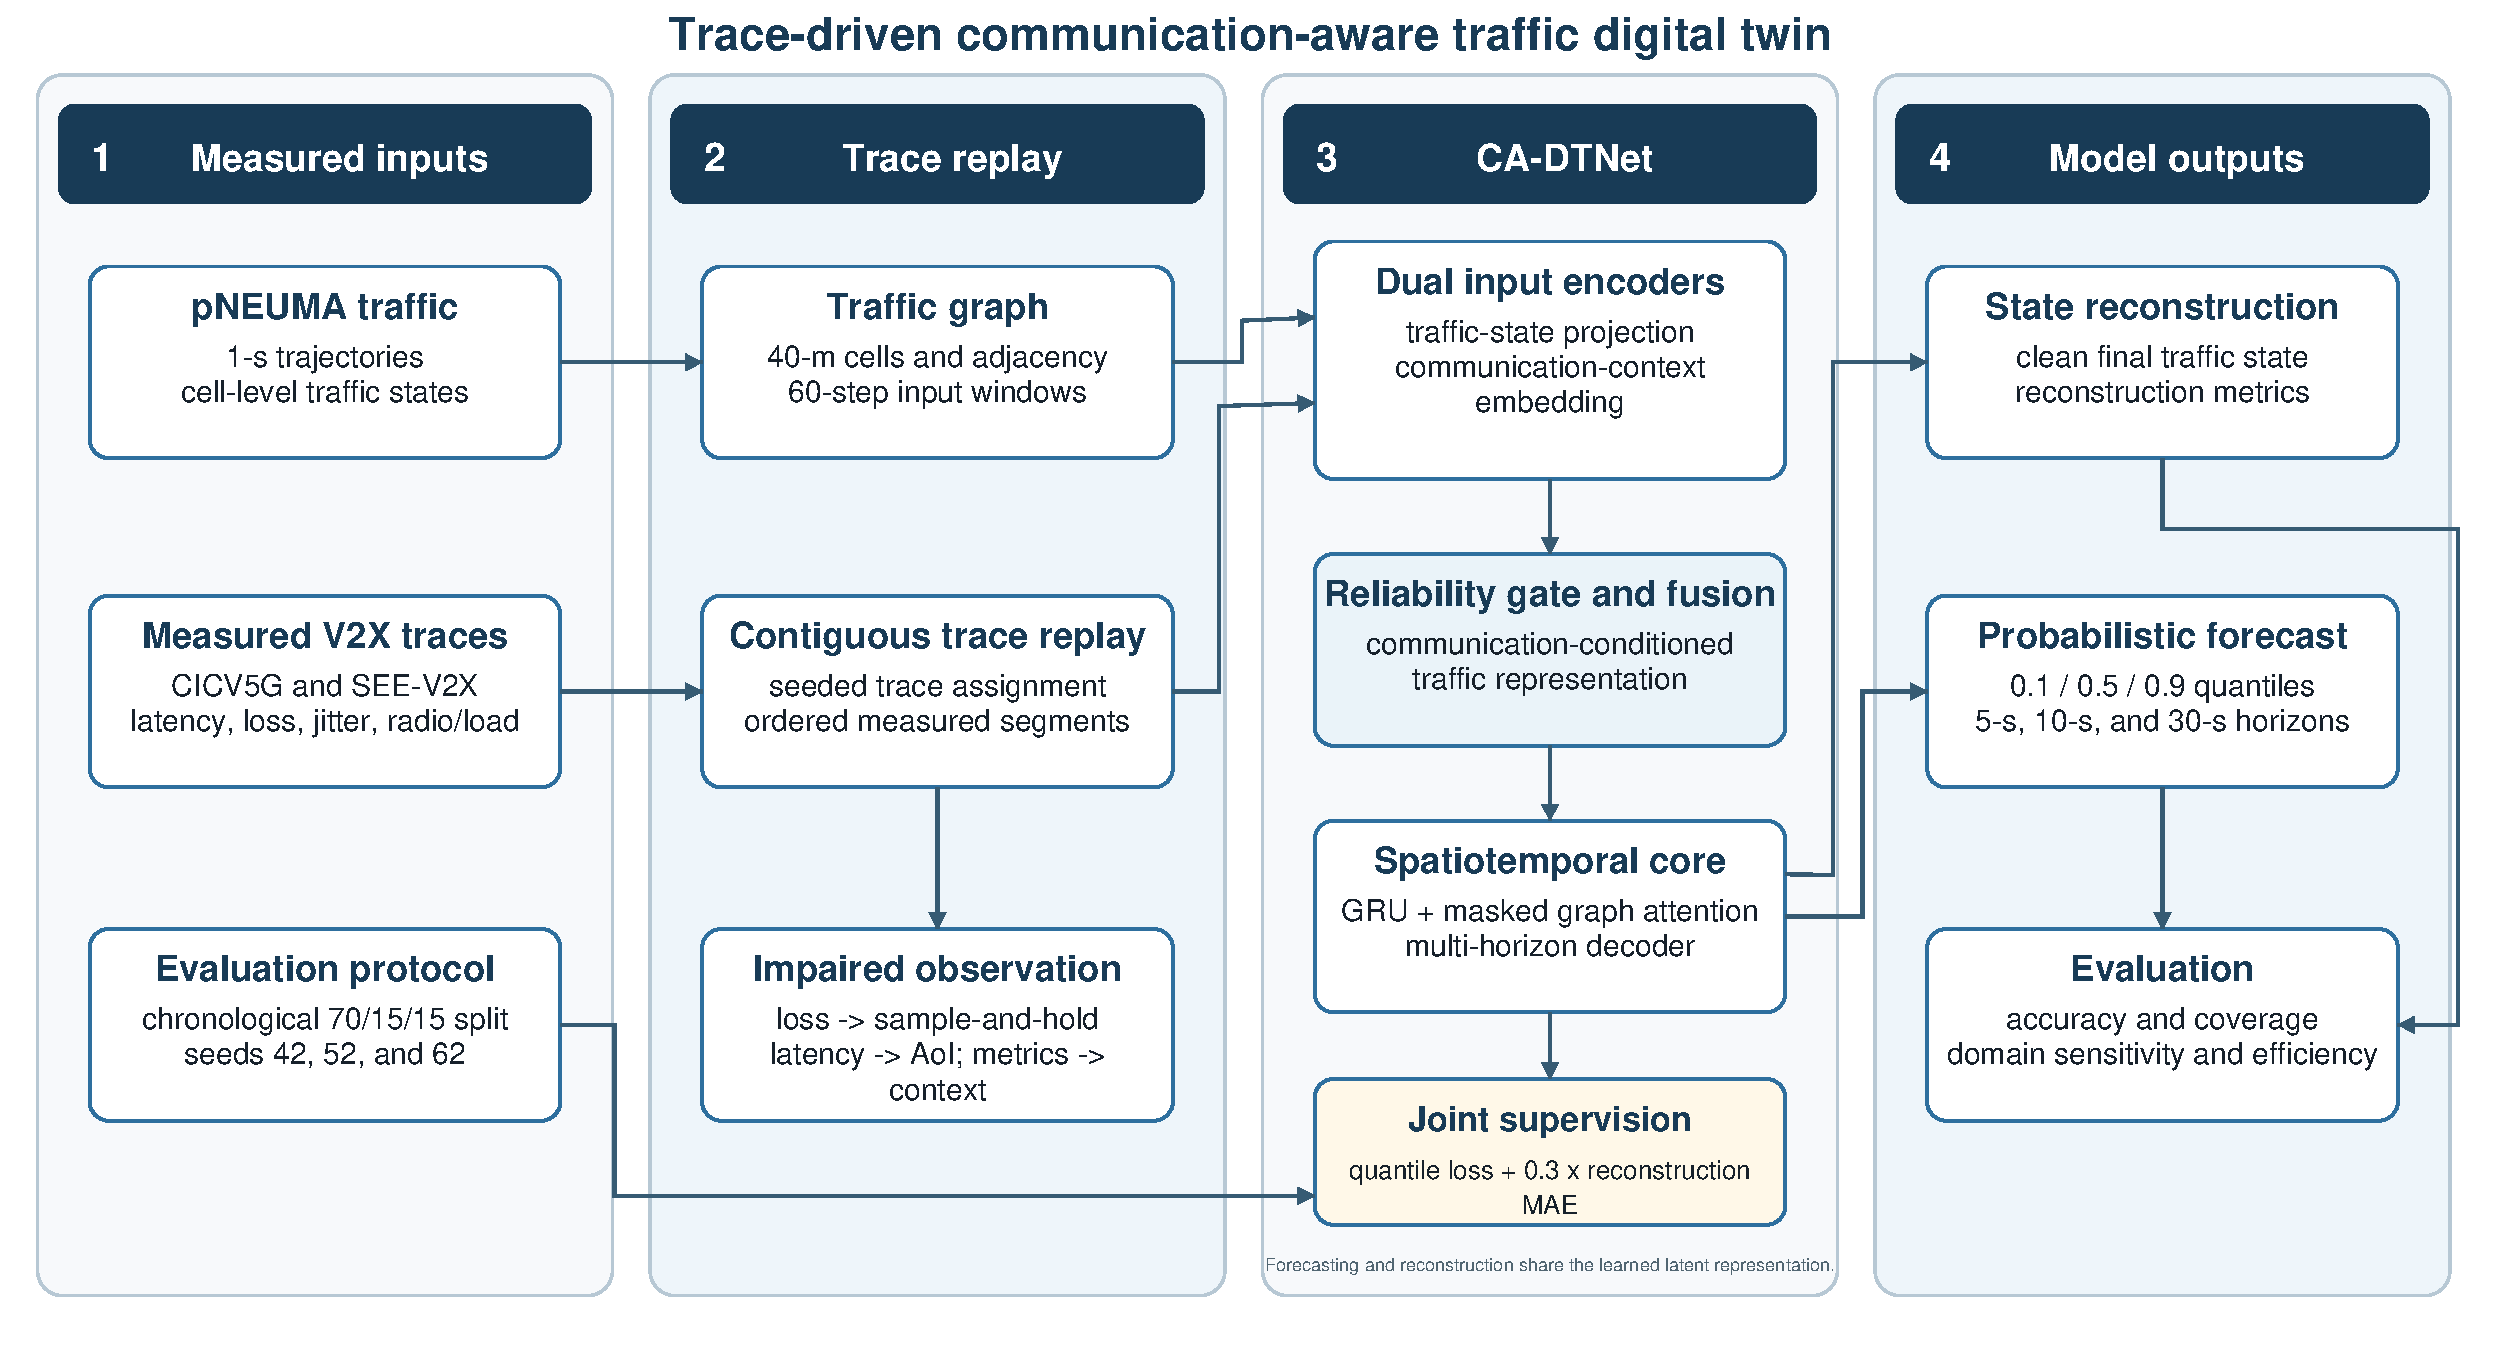
\includegraphics[width=1.00\textwidth]{Fig1_CA_DTNet_architecture.pdf}
    \caption{\change{End-to-end CA-DTNet workflow. Ordered pNEUMA states and measured CICV5G/SEE-V2X trace segments enter a deterministic replay stage. Packet delivery controls the sample-and-hold observation and AoI evolution; the remaining measured network variables form communication context. Traffic projection, reliability gating, temporal encoding, and graph-masked attention produce a shared latent state used for clean-state reconstruction and 0.1/0.5/0.9 quantile forecasts at 5, 10, and 30~s. The four-stage layout separates measured inputs, replay, learning, and outputs to make the information flow explicit.}}
    \label{fig:ca_dtnet_architecture}
\end{figure}

\subsection{Overview of CA-DTNet}
\label{subsec:cadtnet_overview}

The proposed framework is designed around four modelling requirements. First, the model should capture high resolution temporal traffic dynamics from one second traffic histories. Second, it should explicitly represent the communication condition through which the traffic observation is received. Third, it should learn spatial interaction among road segments through a graph based representation. Fourth, it should support both digital twin state reconstruction and probabilistic multi horizon forecasting.

Let the communication impaired traffic sequence be denoted by
\begin{equation}
    \widetilde{\mathbf{X}}_{t-T+1:t},
\end{equation}
where \(T\) is the look back window length. Let the corresponding communication context be
\begin{equation}
    \mathbf{C}_{t-T+1:t}.
\end{equation}
The traffic graph is represented by the adjacency matrix
\begin{equation}
    \mathbf{A}.
\end{equation}
CA-DTNet learns a mapping of the form
\begin{equation}
    f_{\Theta}
    \left(
    \widetilde{\mathbf{X}}_{t-T+1:t},
    \mathbf{C}_{t-T+1:t},
    \mathbf{A}
    \right)
    =
    \left(
    \widehat{\mathbf{X}}_{t},
    \left\{
    \widehat{\mathbf{Y}}_{t+\tau}^{q}
    \right\}_{\tau\in\mathcal{H}, q\in\mathcal{Q}}
    \right),
\end{equation}
where \(\Theta\) denotes the trainable parameters, \(\widehat{\mathbf{X}}_{t}\) is the reconstructed clean traffic state, and \(\widehat{\mathbf{Y}}_{t+\tau}^{q}\) is the predicted traffic quantile at horizon \(\tau\) and quantile level \(q\). The horizon set is
\begin{equation}
    \mathcal{H} = \left\{5, 10, 30\right\},
\end{equation}
and the quantile set is
\begin{equation}
    \mathcal{Q} = \left\{0.10, 0.50, 0.90\right\}.
\end{equation}

As shown in Fig.~\ref{fig:ca_dtnet_architecture}, the model contains six functional blocks: traffic feature projection, communication-context encoding and reliability gating, temporal encoding, graph-masked spatial attention, digital-twin refinement, and the reconstruction and probabilistic forecasting heads. The uncluttered left-to-right organization also distinguishes measured inputs from the replay transformation, preventing the communication trace from being mistaken for a geographically co-located traffic sensor stream.

\begin{changed}
\subsection{Traffic projection and temporal encoder}
\label{subsec:traffic_temporal_encoder}

The released implementation first maps each eight-dimensional impaired traffic vector into a 64-dimensional state using a linear layer, layer normalization, and GELU activation:
\begin{equation}
\mathbf{h}^{x}_{i,k}=\mathrm{GELU}\!\left(\mathrm{LN}\!\left(\mathbf{W}_{x}\widetilde{\mathbf{x}}_{i,k}+\mathbf{b}_{x}\right)\right).
\end{equation}
Temporal recurrence is applied after communication gating, rather than through a separate pre-fusion traffic GRU. This ordering matches the released model and ensures that every step entering the recurrent encoder already reflects its communication reliability.

\subsection{Communication encoder and reliability gate}
\label{subsec:communication_encoder}

Each 27-dimensional prepared communication/context vector is mapped to the traffic hidden width by a two-layer feed-forward encoder with layer normalization, GELU, dropout, and a sigmoid output:
\begin{equation}
\mathbf{h}^{c}_{i,k}=\sigma\!\left(\mathbf{W}_{c2}\,\mathrm{Dropout}\!\left(\mathrm{GELU}\!\left(\mathrm{LN}\!\left(\mathbf{W}_{c1}\mathbf{c}_{i,k}+\mathbf{b}_{c1}\right)\right)\right)+\mathbf{b}_{c2}\right).
\end{equation}
A second sigmoid layer produces an element-wise reliability vector
\begin{equation}
\mathbf{r}_{i,k}=\sigma\!\left(\mathbf{W}_{g}\mathbf{h}^{c}_{i,k}+\mathbf{b}_{g}\right).
\end{equation}
The encoder does not predict communication variables. It converts the measured context into a soft reliability mask used to interpret the received traffic vector.

\subsection{Communication-aware fusion}
\label{subsec:communication_fusion}

Let \(\mathbf{e}_i\) be the learned embedding of road node \(i\). Fusion is performed by
\begin{equation}
\mathbf{u}_{i,k}=\mathbf{h}^{x}_{i,k}\odot\mathbf{r}_{i,k}+\mathbf{e}_{i},
\end{equation}
where \(\odot\) denotes element-wise multiplication. The reliability gate can suppress or retain individual hidden features according to the contemporaneous communication context, while the node embedding retains location-specific structure. A shared GRU then summarizes the gated 60-step sequence:
\begin{equation}
\mathbf{h}^{T}_{i,t}=\mathrm{GRU}\!\left(\mathbf{u}_{i,t-T+1:t}\right).
\end{equation}

\subsection{Graph-masked spatial attention and twin refinement}
\label{subsec:graph_attention_encoder}

CA-DTNet uses single-head scaled dot-product attention constrained by the road adjacency matrix. Self-links are added to the mask. For nodes \(i\) and \(j\),
\begin{equation}
s_{ij}=\frac{(\mathbf{W}_{Q}\mathbf{h}^{T}_{i,t})^{\top}(\mathbf{W}_{K}\mathbf{h}^{T}_{j,t})}{\sqrt{d}},
\qquad
\alpha_{ij}=\frac{\exp(s_{ij})}{\sum_{\ell\in\mathcal{N}(i)\cup\{i\}}\exp(s_{i\ell})},
\end{equation}
with \(s_{ij}=-\infty\) outside \(\mathcal{N}(i)\cup\{i\}\). The residual spatial state is
\begin{equation}
\mathbf{h}^{S}_{i,t}=\mathrm{LN}\!\left(\mathbf{h}^{T}_{i,t}+\mathbf{W}_{O}\sum_{j}\alpha_{ij}\mathbf{W}_{V}\mathbf{h}^{T}_{j,t}\right).
\end{equation}
Temporal and spatial states are concatenated and passed through a two-layer refinement network,
\begin{equation}
\mathbf{h}^{DT}_{i,t}=\mathrm{LN}\!\left(\mathbf{W}_{2}\,\mathrm{Dropout}\!\left(\mathrm{GELU}\!\left(\mathbf{W}_{1}[\mathbf{h}^{T}_{i,t}\Vert\mathbf{h}^{S}_{i,t}]+\mathbf{b}_{1}\right)\right)+\mathbf{b}_{2}\right),
\end{equation}
which is the shared digital-twin representation consumed by both output heads. This specification matches the repository implementation and makes the source of shared supervision explicit.
\end{changed}

\subsection{Digital twin reconstruction head}
\label{subsec:reconstruction_head}

The reconstruction head estimates the clean present traffic state from the shared refined representation. This output is necessary because a digital twin should maintain a physically meaningful representation of the current system state even when the received observation is impaired.

The reconstructed clean state is computed from the shared digital-twin state as
\begin{equation}
    \widehat{\mathbf{X}}_{t}
    =
    \mathbf{W}_{r}
    \mathbf{H}^{DT}_{t}
    +
    \mathbf{b}_{r},
\end{equation}
where \(\mathbf{W}_{r}\) and \(\mathbf{b}_{r}\) are trainable parameters.

The reconstruction loss is
\begin{equation}
    \mathcal{L}_{rec}
    =
    \frac{1}{N F}
    \sum_{i=1}^{N}
    \sum_{k=1}^{F}
    \left|
    X_{i,t}^{k}
    -
    \widehat{X}_{i,t}^{k}
    \right|.
\end{equation}

This loss encourages the shared representation to remain consistent with the physical traffic state. It also prevents the model from learning a representation that is useful only for point prediction but weak for digital twin state recovery.

\subsection{Probabilistic multi horizon forecasting head}
\label{subsec:forecasting_head}

The forecasting head emits all horizon--target--quantile combinations through one linear layer. For each horizon \(\tau\in\mathcal{H}\) and quantile level \(q\in\mathcal{Q}\), the reshaped output is
\begin{equation}
    \widehat{\mathbf{Y}}_{t+\tau}^{q}
    =
    \mathbf{W}_{f}^{(\tau,q)}
    \mathbf{H}^{DT}_{t}
    +
    \mathbf{b}_{f}^{(\tau,q)},
\end{equation}
where \(\mathbf{W}_{f}^{(\tau,q)}\) and \(\mathbf{b}_{f}^{(\tau,q)}\) denote the corresponding slice of the shared forecast head.

The median prediction is obtained from \(q=0.50\). The lower and upper bounds of the prediction interval are obtained from \(q=0.10\) and \(q=0.90\), respectively. Therefore, the model provides both a point forecast and an uncertainty interval.

For a target value \(\mathbf{Y}_{t+\tau}\), the quantile loss is
\begin{equation}
    \rho_q
    \left(
    \mathbf{Y}_{t+\tau}
    -
    \widehat{\mathbf{Y}}_{t+\tau}^{q}
    \right)
    =
    \max
    \left(
    q
    \left(
    \mathbf{Y}_{t+\tau}
    -
    \widehat{\mathbf{Y}}_{t+\tau}^{q}
    \right),
    \left(q-1\right)
    \left(
    \mathbf{Y}_{t+\tau}
    -
    \widehat{\mathbf{Y}}_{t+\tau}^{q}
    \right)
    \right).
\end{equation}

The complete quantile forecasting loss is
\begin{equation}
    \mathcal{L}_{q}
    =
    \frac{1}{|\mathcal{H}|\,|\mathcal{Q}|}
    \sum_{\tau\in\mathcal{H}}
    \sum_{q\in\mathcal{Q}}
    \rho_q
    \left(
    \mathbf{Y}_{t+\tau}
    -
    \widehat{\mathbf{Y}}_{t+\tau}^{q}
    \right).
\end{equation}

The quantile formulation is suitable for this study because it does not require a fixed Gaussian error assumption and can represent asymmetric uncertainty.

\subsection{Joint optimization}
\label{subsec:joint_optimization}

CA-DTNet is trained using a joint multi task objective:
\begin{equation}
    \mathcal{L}
    =
    \lambda_{q}\mathcal{L}_{q}
    +
    \lambda_{r}\mathcal{L}_{rec},
\end{equation}
where \(\lambda_q=1.0\) and \(\lambda_r=0.3\) in every reported CA-DTNet run. The reconstruction term is intentionally auxiliary; the no-reconstruction ablation is the endpoint \(\lambda_r=0\).

The forecasting objective trains the model to predict future traffic states with uncertainty estimates. The reconstruction objective trains the model to recover the clean present state. Since both heads share the traffic projection, communication reliability gate, temporal GRU, graph-masked attention, and twin-refinement layers, the learned latent representation is encouraged to support both digital-twin synchronization and future prediction.

\subsection{Training procedure}
\label{subsec:training_procedure}

The model is trained using mini batch gradient based optimization. Each mini batch contains impaired traffic histories, communication histories, clean current states, and future traffic targets. The training procedure is summarised in Algorithm~\ref{alg:cadtnet_training}.

\begin{algorithm}[htbp]
\caption{Training procedure of CA-DTNet}
\label{alg:cadtnet_training}
\begin{algorithmic}[1]
\Require Traffic graph \(\mathcal{G}\), adjacency matrix \(\mathbf{A}\), impaired traffic sequence \(\widetilde{\mathbf{X}}_{t-T+1:t}\), communication sequence \(\mathbf{C}_{t-T+1:t}\), clean traffic state \(\mathbf{X}_{t}\), future target \(\mathbf{Y}_{t+\tau}\), horizon set \(\mathcal{H}\), quantile set \(\mathcal{Q}\)
\Ensure Trained model parameters \(\Theta\)
\State Initialize all trainable parameters \(\Theta\)
\For{each training epoch}
    \For{each mini batch}
        \State Encode impaired traffic histories using the traffic temporal encoder
        \State Encode communication histories using the communication encoder
        \State Fuse traffic and communication representations using the gating module
        \State Apply graph attention over the traffic graph
        \State Reconstruct the clean digital twin state \(\widehat{\mathbf{X}}_{t}\)
        \State Predict quantile forecasts \(\widehat{\mathbf{Y}}_{t+\tau}^{q}\) for all \(\tau\in\mathcal{H}\) and \(q\in\mathcal{Q}\)
        \State Compute reconstruction loss \(\mathcal{L}_{rec}\)
        \State Compute quantile forecasting loss \(\mathcal{L}_{q}\)
        \State Compute joint loss \(\mathcal{L}=\lambda_{q}\mathcal{L}_{q}+\lambda_{r}\mathcal{L}_{rec}\)
        \State Update \(\Theta\) using gradient based optimization
    \EndFor
\EndFor
\State \Return \(\Theta\)
\end{algorithmic}
\end{algorithm}

\subsection{Inference procedure}
\label{subsec:inference_procedure}

During inference, the trained model receives the latest impaired traffic history and communication history. It produces the reconstructed clean state
\begin{equation}
    \widehat{\mathbf{X}}_{t},
\end{equation}
and the set of future quantile forecasts
\begin{equation}
    \left\{
    \widehat{\mathbf{Y}}_{t+\tau}^{0.10},
    \widehat{\mathbf{Y}}_{t+\tau}^{0.50},
    \widehat{\mathbf{Y}}_{t+\tau}^{0.90}
    \right\}_{\tau\in\mathcal{H}}.
\end{equation}

The median output is used for point forecasting evaluation, while the lower and upper quantiles define the prediction interval. The same trained model is evaluated under clean, CICV5G, and SEE V2X domains. This permits a direct assessment of both forecasting performance and communication domain stability.

\subsection{Methodological connection with the research objective}
\label{subsec:methodological_connection}

The proposed methodology is directly aligned with the research gap identified in Section~\ref{sec:related_work}. The traffic temporal encoder captures short term mobility dynamics. The communication encoder represents observation reliability and information freshness. The fusion module integrates both views into a communication aware latent state. The graph attention encoder models spatial relations over the road network. The reconstruction head supports the digital twin requirement by recovering the clean present state. The probabilistic forecasting head supports reliable prediction by estimating both median forecasts and uncertainty intervals.

Thus, CA-DTNet is not a conventional traffic forecasting model with additional communication variables. It is a communication aware digital twin framework that jointly learns present state reconstruction, graph based traffic forecasting, and uncertainty estimation under measured vehicular communication conditions.

\section{Experimental Setup}
\label{sec:experimental_setup}

This section describes the datasets, trace driven preprocessing, model variants, baselines, evaluation domains, metrics, and implementation settings used to evaluate CA-DTNet. The experimental design follows the system model in Section~\ref{sec:system_model} and the methodology in Section~\ref{sec:methodology}. The main objective is to evaluate whether a communication aware digital twin can reconstruct the clean traffic state, forecast future traffic states, quantify uncertainty, and remain stable under heterogeneous vehicular communication conditions.

\subsection{Datasets}
\label{subsec:datasets}

\begin{changed}
The experimental study deliberately combines one high-resolution traffic source with two vehicular communication sources. pNEUMA was selected because its drone trajectories provide lane-level vehicle motion at sufficient temporal resolution to construct one-second node states, whereas commonly used loop-detector benchmarks cannot reproduce vehicle-level state aggregation at this resolution. CICV5G and SEE-V2X were selected because they expose measured, time-ordered communication variables rather than only summary channel models, and because their different radio and traffic conditions support matched domain comparison.

The three datasets are complementary rather than geographically synchronized. pNEUMA supplies the physical mobility process; CICV5G and SEE-V2X supply measured network stress sequences. This separation allows controlled replay without arbitrary Gaussian corruption, but it also limits inference: the experiments establish robustness for Athens-derived traffic states under two available communication trace families, not universal geographic or network generalization. Section~\ref{subsec:discussion_limitations} states this boundary explicitly.
\end{changed}

\begin{table}[!htbp]
\caption{Datasets used in the experimental study.}
\label{tab:datasets}

\centering
\footnotesize
\renewcommand{\arraystretch}{1.15}
\setlength{\tabcolsep}{3pt}

\begin{tabularx}{\linewidth}{
>{\RaggedRight\arraybackslash}p{2.0cm}
>{\RaggedRight\arraybackslash}p{2.4cm}
>{\RaggedRight\arraybackslash}X
>{\RaggedRight\arraybackslash}p{2.5cm}
}

\toprule

\textbf{Dataset} &
\textbf{Role in This Study} &
\textbf{Main Information Used} &
\textbf{Purpose} \\

\midrule

pNEUMA
&
Physical traffic source
&
One-second vehicle trajectories, speed, vehicle count, traffic flow proxy, and spatial traffic units.
&
Construction of clean traffic states and traffic graph. \\

CICV5G
&
Communication dataset
&
Latency, Age of Information (AoI), packet loss, jitter, throughput, signal strength, signal quality, and channel condition.
&
Generation of CICV5G-impaired traffic observations. \\

SEE V2X
&
Communication dataset
&
Latency, Age of Information (AoI), packet loss, jitter, throughput, signal strength, signal quality, and channel condition.
&
Generation of SEE V2X-impaired traffic observations. \\

\bottomrule

\multicolumn{4}{p{\dimexpr\linewidth-2\tabcolsep\relax}}{\footnotesize
\textbf{Abbreviations:}
AoI = Age of Information;
V2X = Vehicle-to-Everything.
The pNEUMA dataset provides the physical traffic measurements used to construct clean traffic states, whereas the CICV5G and SEE V2X datasets provide communication-quality indicators for modelling communication-impaired traffic observations.
}

\end{tabularx}

\end{table}
\subsection{Traffic state construction}
\label{subsec:traffic_state_construction}

The pNEUMA trajectories are first transformed into regularly sampled traffic states. Each traffic state is generated at one second resolution. The road environment is divided into spatial traffic units, and each unit is treated as a graph node. For each node and time instant, three primary traffic variables are computed:
\begin{equation}
    \mathbf{x}_{i,t}
    =
    \left[
    v_{i,t},
    n_{i,t},
    f_{i,t}
    \right],
\end{equation}
where \(v_{i,t}\) is the mean speed, \(n_{i,t}\) is the vehicle count, and \(f_{i,t}\) is the flow proxy.

The graph adjacency matrix \(\mathbf{A}\) is constructed from the spatial relation among traffic units. The resulting graph allows the model to learn the dependence among neighbouring or functionally related road segments. Each training sample contains a historical traffic window and future traffic targets at multiple horizons.

\subsection{Communication trace replay}
\label{subsec:communication_trace_replay}

\begin{changed}
The implementation follows the procedure formalized in Section~\ref{sec:system_model}. Traffic is binned at 1~s. Communication rows are ordered by trace identifier and sample index; one contiguous, seeded segment is assigned to each traffic node by index rather than by geographic coordinates. At each aligned step, the measured loss probability controls a Bernoulli delivery event. A successful delivery updates the received state and resets AoI to the capped measured latency; a failed delivery holds the last received traffic state and increments AoI by the one-second bin duration. Jitter, load, throughput, RSRP, SINR, and standardized latency/loss values remain contextual inputs to the reliability gate.

This replay produces three observation domains:
\begin{equation}
    \mathcal{D}^{clean},
    \quad
    \mathcal{D}^{cic},
    \quad
    \mathcal{D}^{see}.
\end{equation}

The clean domain \(\mathcal{D}^{clean}\) contains the original traffic observations; \(\mathcal{D}^{cic}\) and \(\mathcal{D}^{see}\) use the respective replayed sequences. The same replay realization is supplied to every model, and the assignment is independent of traffic targets and model errors. Chronological 70/15/15 splitting is performed without shuffling, and all scalers are fitted to the training partition only. Therefore, the held-out windows contain unseen temporal segments, although the identities of the two communication datasets are known during training.
\end{changed}

\begin{table}[htbp]
\centering
\caption{Communication variables used as contextual inputs.}
\label{tab:communication_variables}
\small
\begin{tabularx}{\linewidth}{p{2.5cm} X p{3.0cm}}
\hline
Variable & Interpretation & Relevance to CA-DTNet \\
\hline
Latency & Time required for a message or observation to reach the receiver & Indicates delayed observation delivery \\
Age of information & Time elapsed since the generation of the latest received update & Measures freshness of the received traffic state \\
Packet loss & Fraction or indicator of missing communication packets & Represents incomplete observation transfer \\
Jitter & Variation in delay across received messages & Indicates temporal irregularity in updates \\
Channel busy ratio & Occupancy or congestion of the wireless channel & Represents communication contention \\
Throughput & Effective data transfer rate & Indicates available communication capacity \\
RSRP & Received signal reference power & Represents signal strength \\
SINR & Signal to interference plus noise ratio & Represents signal quality \\
\hline
\end{tabularx}
\end{table}

\subsection{Input and output configuration}
\label{subsec:input_output_configuration}

Each model receives a historical traffic sequence and predicts future traffic targets. CA-DTNet additionally receives the communication context aligned with the same historical window. The forecasting horizons are
\begin{equation}
    \mathcal{H}
    =
    \left\{5, 10, 30\right\}
    \text{ seconds}.
\end{equation}
The target variables are speed, vehicle count, and flow proxy.

For probabilistic forecasting, CA-DTNet predicts three quantile levels:
\begin{equation}
    \mathcal{Q}
    =
    \left\{0.10, 0.50, 0.90\right\}.
\end{equation}
The median quantile is used as the point forecast, while the lower and upper quantiles form the prediction interval.

\begin{table}[htbp]
\centering
\caption{Forecasting configuration.}
\label{tab:forecasting_configuration}
\small
\begin{tabular}{p{4.0cm} p{7.0cm}}
\hline
Item & Configuration \\
\hline
Traffic resolution & One second \\
Traffic targets & Speed, vehicle count, and flow proxy \\
Forecasting horizons & Five seconds, ten seconds, and thirty seconds \\
Observation domains & Clean, CICV5G impaired, and SEE V2X impaired \\
Probabilistic outputs & Quantiles at 0.10, 0.50, and 0.90 \\
Point forecast & Median quantile at 0.50 \\
Prediction interval & Interval between 0.10 and 0.90 quantiles \\
\hline
\end{tabular}
\end{table}

\subsection{Models compared}
\label{subsec:models_compared}

The proposed CA-DTNet is compared with three graph based forecasting baselines and several ablated versions of the proposed model. The baseline models are selected because they represent common spatial temporal forecasting families. DCRNN represents diffusion based recurrent graph forecasting. Graph WaveNet represents adaptive graph and dilated temporal convolution based forecasting. Graph GRU represents a compact graph recurrent forecasting baseline.

The comparison is designed to evaluate whether the proposed communication aware digital twin framework provides benefits beyond standard graph temporal modelling. The same train, validation, and test protocol is used across the learned models.

\begin{table}[!htbp]
\caption{Forecasting models used in the comparative evaluation.}
\label{tab:models_compared}

\centering
\footnotesize
\renewcommand{\arraystretch}{1.15}
\setlength{\tabcolsep}{3pt}

\begin{tabularx}{\linewidth}{
>{\RaggedRight\arraybackslash}p{2.3cm}
>{\RaggedRight\arraybackslash}X
>{\RaggedRight\arraybackslash}p{2.5cm}
}

\toprule

\textbf{Model} &
\textbf{Main Modelling Characteristic} &
\textbf{Role in Evaluation} \\

\midrule

DCRNN
&
Diffusion-based graph recurrent neural network for spatio-temporal traffic forecasting.
&
Strong graph recurrent baseline. \\

Graph WaveNet
&
Adaptive graph learning with dilated temporal convolution for spatial and temporal dependency modelling.
&
Strong graph convolution baseline. \\

Graph GRU
&
Compact graph recurrent forecasting architecture with reduced computational complexity.
&
Efficient graph recurrent baseline. \\

\textbf{CA-DTNet}
&
Communication-aware traffic encoding, graph attention, digital twin reconstruction, and quantile-based probabilistic forecasting.
&
\textbf{Proposed model}. \\

\bottomrule

\multicolumn{3}{p{\dimexpr\linewidth-2\tabcolsep\relax}}{\footnotesize
\textbf{Abbreviations:}
DCRNN = Diffusion Convolutional Recurrent Neural Network;
GRU = Gated Recurrent Unit.
CA-DTNet integrates communication-aware feature encoding, digital twin state reconstruction, graph attention learning, and probabilistic traffic forecasting within a unified framework.
}

\end{tabularx}

\end{table}

\begin{changed}
Recent Transformer models such as STAEformer, PDFormer, STGformer, STGAFormer, and PatchSTG are discussed in Section~\ref{sec:related_work}. They were not included as numerical baselines because their published formulations operate on clean fixed-sensor benchmarks and do not expose the clean-state reconstruction and measured-communication inputs required for a like-for-like evaluation. Adding their reported numbers would mix datasets, resolutions, targets, and horizons. The controlled experiment instead uses three locally reimplemented graph-temporal families under identical windows, targets, splits, seeds, optimizer settings, and hardware.

Table~\ref{tab:complexity_control} separates model capacity from added supervision. DCRNN and Graph WaveNet contain 1.75 and 1.38 times as many parameters as CA-DTNet, respectively, yet have higher WAPE. Graph GRU is smaller and faster, providing the opposite complexity control. Consequently, the gain cannot be explained by parameter count alone. Component ablations then hold the remaining training protocol fixed to isolate communication encoding, AoI, graph attention, reconstruction, and uncertainty supervision.

\begin{table}[!htbp]
\caption{Complexity-controlled comparison under the common experimental protocol. Parameter ratio is relative to CA-DTNet.}
\label{tab:complexity_control}
\centering
\footnotesize
\begin{tabular}{lrrrr}
\toprule
Model & Parameters & Ratio & WAPE & Latency (ms) \\
\midrule
DCRNN & 124,233 & 1.75 & 0.4393 & 7.4015 \\
Graph WaveNet & 98,541 & 1.38 & 0.4319 & 1.1185 \\
Graph GRU & 34,377 & 0.48 & 0.4403 & 0.1676 \\
CA-DTNet & 71,203 & 1.00 & \textbf{0.4116} & 0.3933 \\
\bottomrule
\end{tabular}
\end{table}
\end{changed}

\subsection{Ablation settings}
\label{subsec:ablation_settings}

Ablation experiments are conducted to study the contribution of each major component of CA-DTNet. The ablated variants remove one component at a time while keeping the remaining model structure as consistent as possible. This design helps identify whether the graph attention module, communication encoder, age of information input, reconstruction objective, and uncertainty objective contribute to the final behaviour of the model.

\begin{table}[!htbp]
\caption{Ablation variants used to evaluate the contribution of individual CA-DTNet components.}
\label{tab:ablation_settings}

\centering
\footnotesize
\renewcommand{\arraystretch}{1.15}
\setlength{\tabcolsep}{3pt}

\begin{tabularx}{\linewidth}{
>{\RaggedRight\arraybackslash}p{2.8cm}
>{\RaggedRight\arraybackslash}X
>{\RaggedRight\arraybackslash}p{2.8cm}
}

\toprule

\textbf{Variant} &
\textbf{Removed Component} &
\textbf{Purpose of Ablation} \\

\midrule

Full CA-DTNet
&
None.
&
Complete proposed model. \\

Without communication encoder
&
Communication representation branch.
&
Evaluates the contribution of communication-aware features. \\

Without Age of Information (AoI)
&
Age of Information feature from the communication context.
&
Assesses the importance of information freshness. \\

Without graph attention
&
Graph attention-based spatial encoder.
&
Evaluates the contribution of spatial dependency learning. \\

Without reconstruction loss
&
Digital twin reconstruction objective.
&
Measures the effect of state reconstruction on prediction performance. \\

Without uncertainty loss
&
Quantile-based uncertainty estimation objective.
&
Evaluates the contribution of probabilistic interval learning. \\

\bottomrule

\multicolumn{3}{p{\dimexpr\linewidth-2\tabcolsep\relax}}{\footnotesize
\textbf{Abbreviations:}
AoI = Age of Information.
Each ablation variant removes a single component of the proposed CA-DTNet framework while keeping all remaining training settings unchanged. This enables an independent assessment of the contribution of each module to forecasting accuracy and uncertainty estimation.
}

\end{tabularx}

\end{table}

The ablation study is interpreted carefully. A component is not assumed to be useful only when it improves every point forecasting metric. For example, communication features may support domain stability and state reconstruction even when a point error metric does not improve in every setting. Therefore, ablation results are evaluated using point forecasting metrics, reconstruction metrics, uncertainty metrics, and communication domain robustness.

\subsection{Training protocol}
\label{subsec:training_protocol}

All learned models are trained using the same general protocol. The training data include communication impaired observations from both CICV5G and SEE V2X domains. This enables the model to learn from heterogeneous communication conditions during training. After training, the models are evaluated separately on clean observations, CICV5G impaired observations, and SEE V2X impaired observations.

To reduce dependence on a single random initialization, the main comparative experiment is repeated using three random seeds:
\begin{equation}
    42,\quad 52,\quad 62.
\end{equation}
The final reported performance is aggregated across these seeds. This makes the comparison more reliable than a single run evaluation.

\begin{table}[htbp]
\centering
\caption{Training and evaluation protocol.}
\label{tab:training_protocol}
\small
\begin{tabular}{p{4.0cm} p{7.0cm}}
\hline
Item & Protocol \\
\hline
Training domains & Combined CICV5G and SEE V2X impaired observations \\
Evaluation domains & Clean, CICV5G, and SEE V2X \\
Random seeds & 42, 52, and 62 \\
Forecasting horizons & Five seconds, ten seconds, and thirty seconds \\
Targets & Speed, vehicle count, and flow proxy \\
Primary comparison & CA-DTNet against DCRNN, Graph WaveNet, and Graph GRU \\
Additional analysis & Ablation, reconstruction, uncertainty, matched domain robustness, and efficiency \\
\hline
\end{tabular}
\end{table}

\begin{changed}
The released CA-DTNet configuration uses 61 nodes, eight prepared traffic features, 27 communication/context features, a 60-step history, hidden width 64, dropout 0.15, batch size 16, Adam with learning rate \(10^{-3}\) and weight decay \(10^{-5}\), gradient-norm clipping at 5.0, and early-stopping patience 6. CA-DTNet is trained for at most 45 epochs; the point baselines use at most 35. Table~\ref{tab:loss_weights} records the loss coefficients used for all seeds.

\begin{table}[!htbp]
\caption{Joint-objective coefficients and selection rule.}
\label{tab:loss_weights}
\centering
\small
\begin{tabular}{p{2.7cm}p{1.7cm}p{7.0cm}}
\toprule
Coefficient & Value & Role and selection \\
\midrule
\(\lambda_q\) & 1.0 & Primary multi-horizon quantile forecasting objective. \\
\(\lambda_r\) & 0.3 & Auxiliary clean-state MAE; fixed from validation behavior to preserve forecasting dominance, with no test-set tuning. \\
Endpoint ablation & 0.0 & Removes reconstruction supervision while retaining the remaining architecture and training protocol. \\
\bottomrule
\end{tabular}
\end{table}
\end{changed}

\subsection{Evaluation metrics}
\label{subsec:evaluation_metrics}

The evaluation uses several metric groups because CA-DTNet has multiple objectives. Point forecasting metrics evaluate prediction accuracy. Reconstruction metrics evaluate the digital twin state recovery capability. Probabilistic metrics evaluate uncertainty quality. Matched domain analysis evaluates communication robustness. Efficiency metrics evaluate practical deployability.

\subsubsection{Point forecasting metrics}

Mean absolute error is defined as
\begin{equation}
    \mathrm{MAE}
    =
    \frac{1}{S}
    \sum_{s=1}^{S}
    \left|
    y_s - \widehat{y}_s
    \right|,
\end{equation}
where \(S\) is the number of evaluated samples, \(y_s\) is the true value, and \(\widehat{y}_s\) is the predicted value.

Root mean square error is defined as
\begin{equation}
    \mathrm{RMSE}
    =
    \sqrt{
    \frac{1}{S}
    \sum_{s=1}^{S}
    \left(
    y_s - \widehat{y}_s
    \right)^2
    }.
\end{equation}

Weighted absolute percentage error is defined as
\begin{equation}
    \mathrm{WAPE}
    =
    \frac{
    \sum_{s=1}^{S}
    \left|
    y_s - \widehat{y}_s
    \right|
    }{
    \sum_{s=1}^{S}
    \left|
    y_s
    \right|
    +
    \epsilon
    },
\end{equation}
where \(\epsilon\) is a small constant used to avoid division by zero.

The coefficient of determination is computed as
\begin{equation}
    R^{2}
    =
    1
    -
    \frac{
    \sum_{s=1}^{S}
    \left(
    y_s - \widehat{y}_s
    \right)^2
    }{
    \sum_{s=1}^{S}
    \left(
    y_s - \bar{y}
    \right)^2
    +
    \epsilon
    },
\end{equation}
where \(\bar{y}\) is the mean of the true values.

\subsubsection{Reconstruction metrics}

The reconstruction head is evaluated by comparing the reconstructed clean state with the actual clean traffic state. The reconstruction evaluation uses WAPE and \(R^{2}\). These metrics indicate whether the digital twin can recover the physical traffic state from impaired observations.

\subsubsection{Probabilistic forecasting metrics}

The prediction interval coverage probability is defined as
\begin{equation}
    \mathrm{PICP}
    =
    \frac{1}{S}
    \sum_{s=1}^{S}
    \mathbb{I}
    \left(
    \widehat{y}_{s}^{0.10}
    \leq
    y_s
    \leq
    \widehat{y}_{s}^{0.90}
    \right),
\end{equation}
where \(\mathbb{I}(\cdot)\) is an indicator function.

The prediction interval normalized average width is defined as
\begin{equation}
    \mathrm{PINAW}
    =
    \frac{1}{S}
    \sum_{s=1}^{S}
    \frac{
    \widehat{y}_{s}^{0.90}
    -
    \widehat{y}_{s}^{0.10}
    }{
    y_{\max} - y_{\min} + \epsilon
    }.
\end{equation}

PICP measures empirical coverage, while PINAW measures interval sharpness. Both are required because very wide intervals may achieve high coverage but may not be useful for decision making.

\subsubsection{Matched communication domain robustness}

Matched domain robustness is evaluated by comparing CICV5G and SEE V2X predictions generated from the same physical traffic window. Let \(e_{s}^{cic}\) be the absolute error under CICV5G and \(e_{s}^{see}\) be the absolute error under SEE V2X for the same matched traffic sample \(s\). The paired error difference is
\begin{equation}
    \Delta e_s
    =
    e_{s}^{see}
    -
    e_{s}^{cic}.
\end{equation}

If a model is stable across communication domains, the paired difference should remain close to zero for most tasks. Statistical testing is used to identify whether the paired difference is significant.

\subsubsection{Efficiency metrics}

Efficiency is evaluated using trainable parameter count, checkpoint size, training time, inference latency, and peak GPU memory. These metrics are important because a communication aware traffic digital twin is expected to operate close to real time.

\subsection{Statistical testing}
\label{subsec:statistical_testing}

The experimental study uses paired statistical tests to compare model errors under matched conditions. The Wilcoxon signed rank test is used because paired sample errors may not follow a normal distribution. The null hypothesis is that the median paired difference between two error samples is zero. A small \(p\) value indicates that the difference is statistically significant.

For communication domain robustness, the Wilcoxon test is applied to matched CICV5G and SEE V2X error samples. For baseline comparison, the test is applied between CA-DTNet and each baseline under the same evaluation domain, target, and forecasting horizon.

\subsection{Implementation details}
\label{subsec:implementation_details}

The models are implemented using a deep learning framework and trained using GPU acceleration. All learned models are trained under the same data split and evaluated using the same test windows. CA-DTNet produces both reconstruction and quantile forecasting outputs. The baseline models produce point forecasts, and their performance is compared using the median output of CA-DTNet.

The final experiment uses three random seeds to report stable comparative performance. The efficiency analysis uses the trained model checkpoints to report parameter count, checkpoint size, inference latency, training time, and memory usage. This ensures that the comparison covers both predictive quality and computational practicality.

\subsection{Summary of experimental design}
\label{subsec:experimental_design_summary}

The experimental design is summarised in Fig.~\ref{fig:experimental_protocol}. The design begins with high resolution pNEUMA traffic state construction and communication trace replay. The resulting clean and impaired domains are used to train and evaluate the models. The evaluation includes point forecasting, digital twin reconstruction, probabilistic forecasting, matched communication robustness, component ablation, and efficiency analysis.

\begin{figure}[htbp]
    \centering
    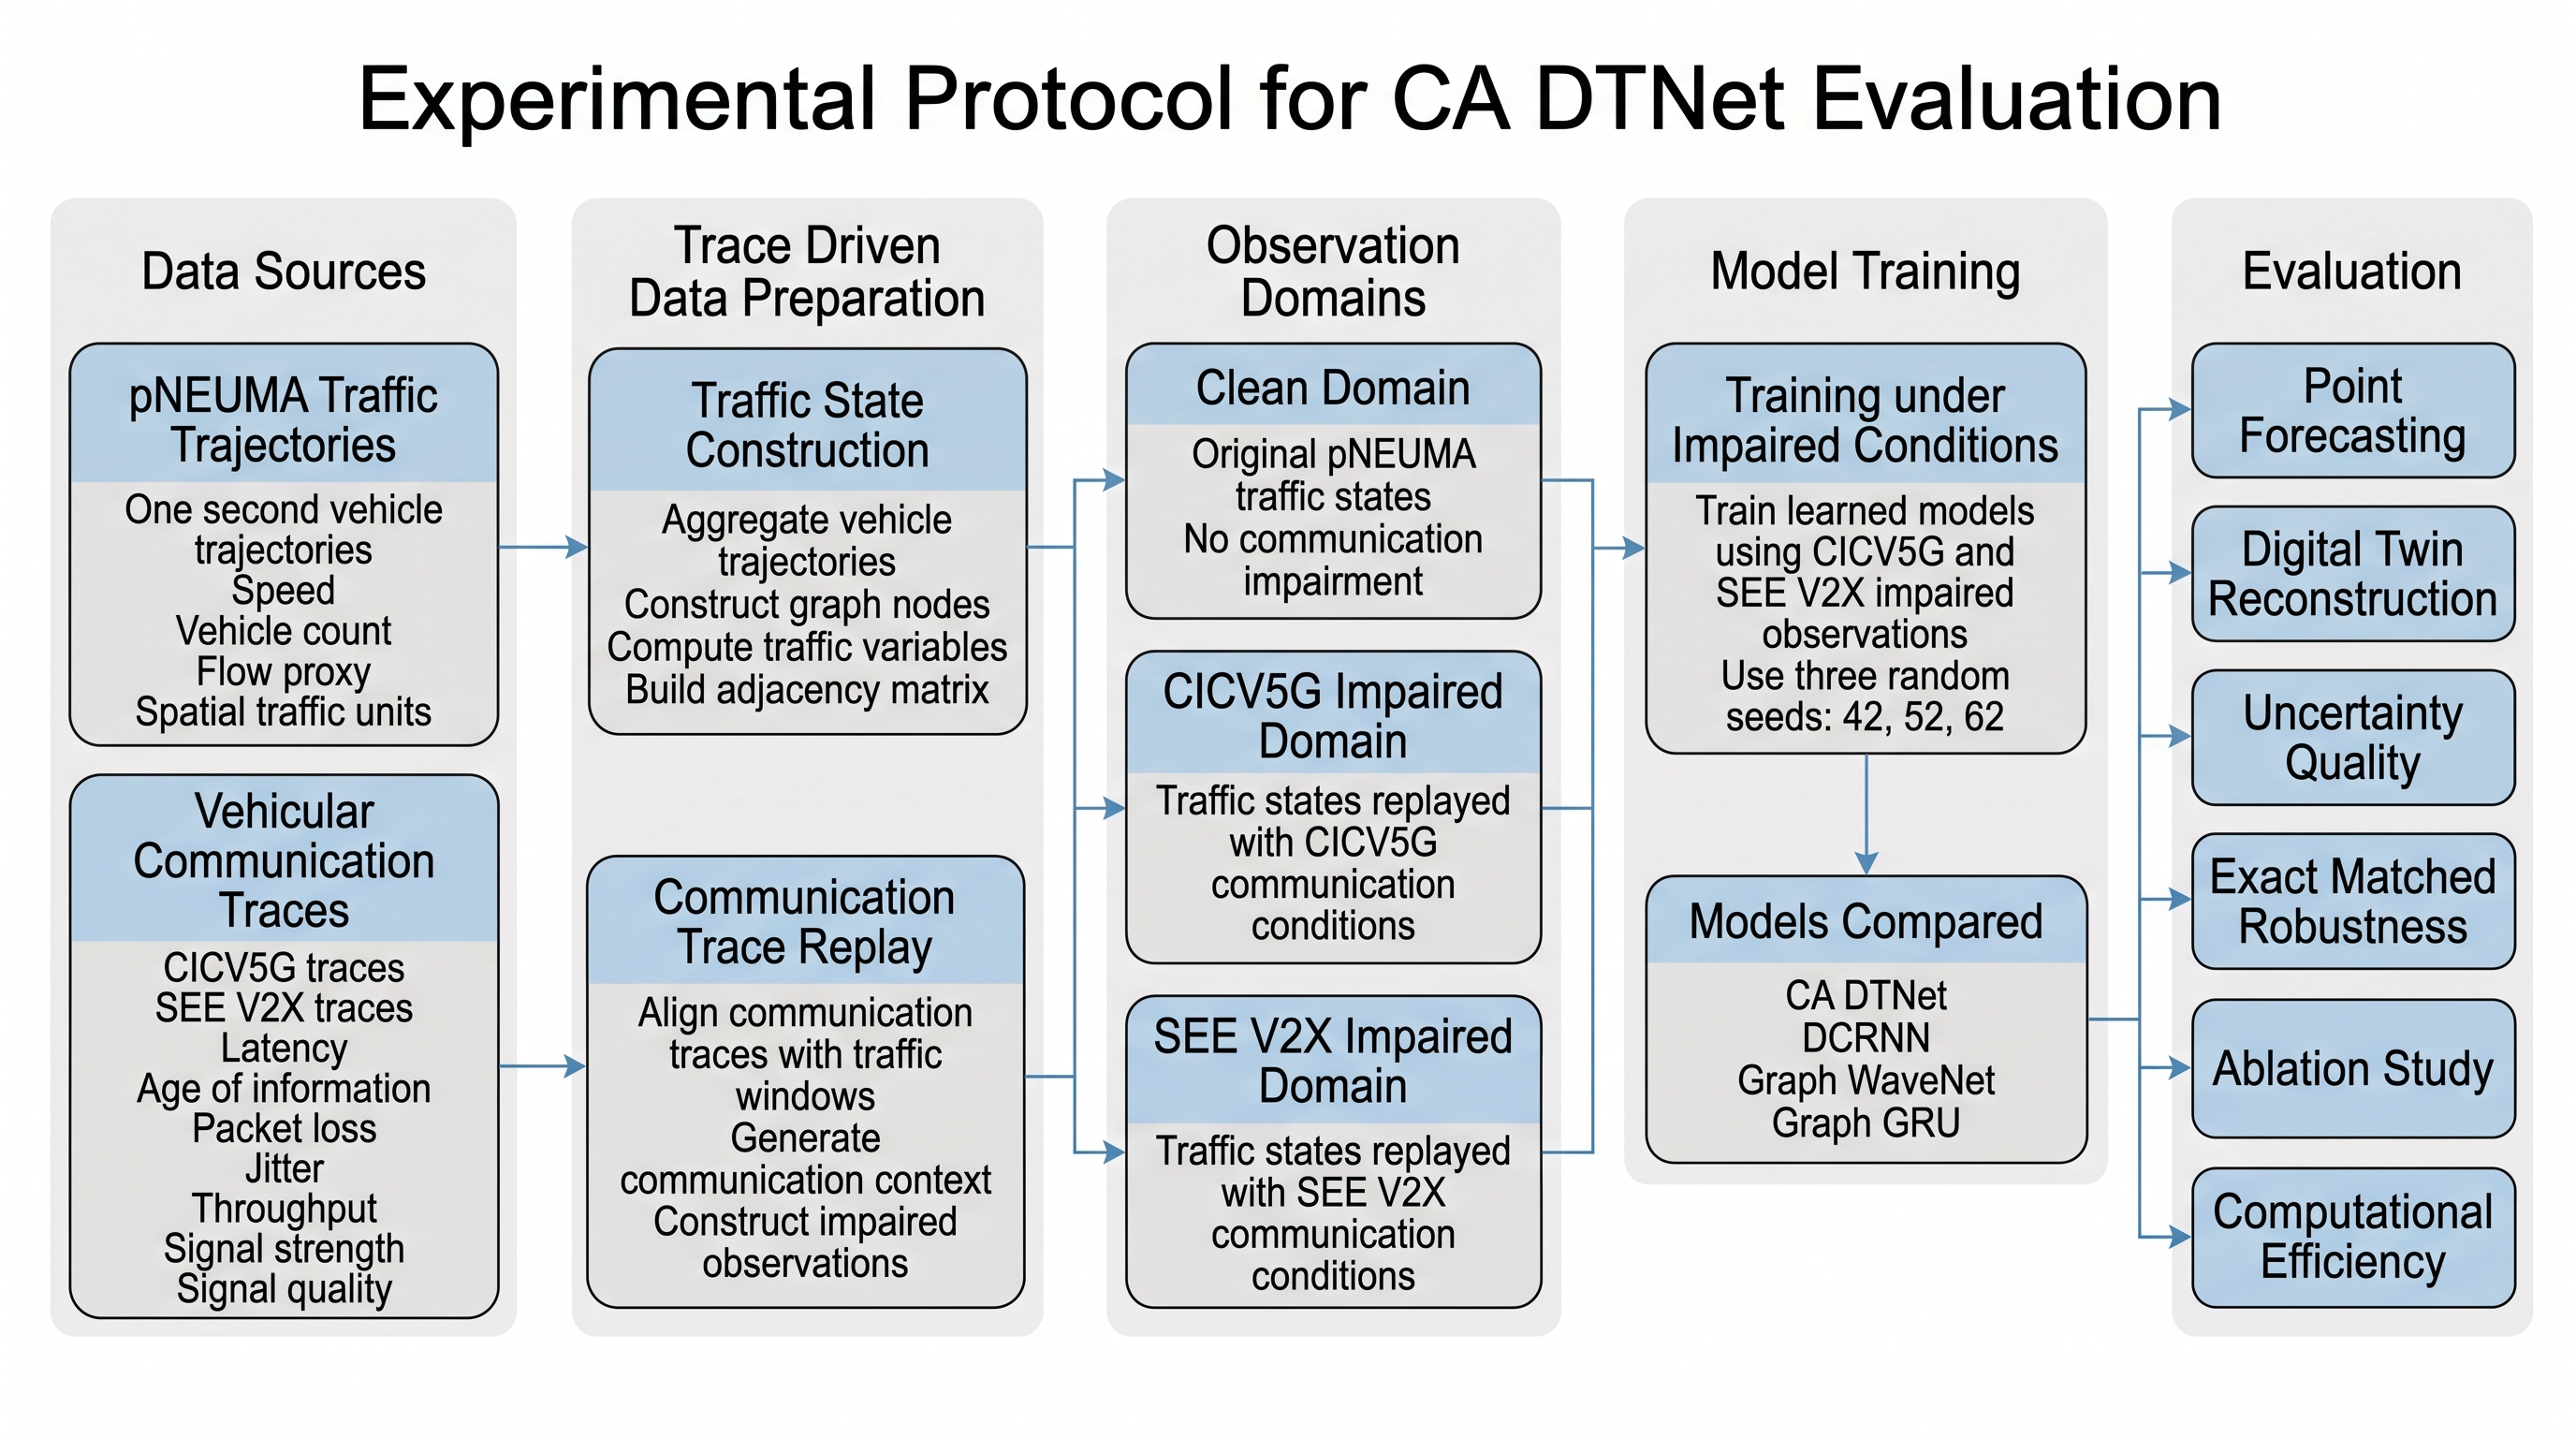
\includegraphics[width=0.98\textwidth]{Fig8_experimental_protocol.jpeg}
    \caption{Experimental protocol used to evaluate CA-DTNet. The pNEUMA traffic states are combined with CICV5G and SEE V2X communication traces to construct clean and impaired observation domains. The learned models are trained under communication impaired conditions and evaluated under clean, CICV5G, and SEE V2X domains. The evaluation covers point forecasting, digital twin reconstruction, uncertainty quality, exact matched communication robustness, ablation, and efficiency.}
    \label{fig:experimental_protocol}
\end{figure}

This setup directly supports the research objective of the paper. It evaluates CA-DTNet not only as a traffic forecasting model, but also as a communication-aware digital twin capable of reconstructing the clean present state and producing reliable multi-horizon forecasts under heterogeneous vehicular communication conditions.

\section{Results and Analysis}
\label{sec:results}

This section presents the experimental results of CA-DTNet and compares its performance with DCRNN, Graph WaveNet, and Graph GRU. The analysis follows the evaluation protocol described in Section~\ref{sec:experimental_setup}. The results are organised into six parts. First, the point forecasting performance is reported across clean, CICV5G, and SEE V2X domains. Second, the statistical comparison with baseline models is discussed. Third, the digital twin reconstruction and probabilistic forecasting results are analysed. Fourth, the matched communication domain robustness is evaluated. Fifth, the component ablation results are presented. Finally, the computational efficiency of the proposed model is discussed.

\subsection{Overall forecasting performance}
\label{subsec:overall_forecasting_performance}

Table~\ref{tab:overall_wape_r2} reports the overall weighted absolute percentage error and coefficient of determination across the three evaluation domains. The results show that CA-DTNet obtains the lowest WAPE in all three domains. This indicates that the proposed model produces lower average percentage error than DCRNN, Graph WaveNet, and Graph GRU under clean observations as well as under communication impaired observations.

\begin{table}[t]
\centering
\caption{Overall forecasting performance across evaluation domains. Lower WAPE is better, while higher \(R^{2}\) is better.}
\label{tab:overall_wape_r2}
\small
\begin{tabular}{p{3.1cm} p{2.5cm} p{2.2cm} p{2.2cm}}
\hline
Model & Domain & WAPE & \(R^{2}\) \\
\hline
CA-DTNet & Clean & 0.4130 & 0.6627 \\
CA-DTNet & CICV5G & 0.4109 & 0.6676 \\
CA-DTNet & SEE V2X & 0.4110 & 0.6677 \\
DCRNN & Clean & 0.4393 & 0.6859 \\
DCRNN & CICV5G & 0.4393 & 0.6859 \\
DCRNN & SEE V2X & 0.4393 & 0.6858 \\
Graph WaveNet & Clean & 0.4318 & 0.6678 \\
Graph WaveNet & CICV5G & 0.4318 & 0.6678 \\
Graph WaveNet & SEE V2X & 0.4322 & 0.6674 \\
Graph GRU & Clean & 0.4401 & 0.6767 \\
Graph GRU & CICV5G & 0.4401 & 0.6767 \\
Graph GRU & SEE V2X & 0.4406 & 0.6761 \\
\hline
\end{tabular}
\end{table}

The WAPE of CA-DTNet remains highly stable across the three domains. The values are 0.4130 in the clean domain, 0.4109 in the CICV5G domain, and 0.4110 in the SEE V2X domain. This stability is important because the model is expected to operate under heterogeneous vehicular communication conditions. The small variation across domains indicates that the proposed communication aware representation does not collapse when the traffic observations are affected by different communication traces.

The improvement of CA-DTNet over the baselines is summarised in Table~\ref{tab:wape_improvement}. The proposed model improves WAPE by approximately 5.99 percent over DCRNN, 4.36 percent over Graph WaveNet, and 6.16 percent over Graph GRU in the clean domain. Under CICV5G impairment, the improvement is 6.46 percent over DCRNN, 4.84 percent over Graph WaveNet, and 6.63 percent over Graph GRU. Under SEE V2X impairment, the improvement is 6.45 percent over DCRNN, 4.90 percent over Graph WaveNet, and 6.72 percent over Graph GRU.

\begin{table}[t]
\centering
\caption{Relative WAPE improvement of CA-DTNet over baseline models.}
\label{tab:wape_improvement}
\small
\begin{tabularx}{\linewidth}{Xccc}
\hline
Domain & Over DCRNN & Over Graph WaveNet & Over Graph GRU \\
\hline
Clean & 5.99 percent & 4.36 percent & 6.16 percent \\
CICV5G & 6.46 percent & 4.84 percent & 6.63 percent \\
SEE V2X & 6.45 percent & 4.90 percent & 6.72 percent \\
\hline
\end{tabularx}
\end{table}

Although CA-DTNet achieves the best WAPE, the \(R^{2}\) results require a balanced interpretation. DCRNN obtains a higher overall \(R^{2}\) than CA-DTNet in all three domains. This means that CA-DTNet is stronger in average absolute and percentage based error reduction, while DCRNN remains competitive in squared error based evaluation. Therefore, the results should not be interpreted as universal dominance of CA-DTNet on every metric. Instead, the proposed model provides a favourable balance among WAPE, communication domain stability, digital twin reconstruction, uncertainty estimation, and computational efficiency.

Figure~\ref{fig:three_seed_forecasting} presents the three seed forecasting comparison. The figure summarises mean WAPE across targets and horizons for clean, CICV5G, and SEE V2X domains. It visually confirms the trend reported in Table~\ref{tab:overall_wape_r2}. CA-DTNet consistently remains below the baseline models in WAPE.

\begin{figure}[htbp]
    \centering
    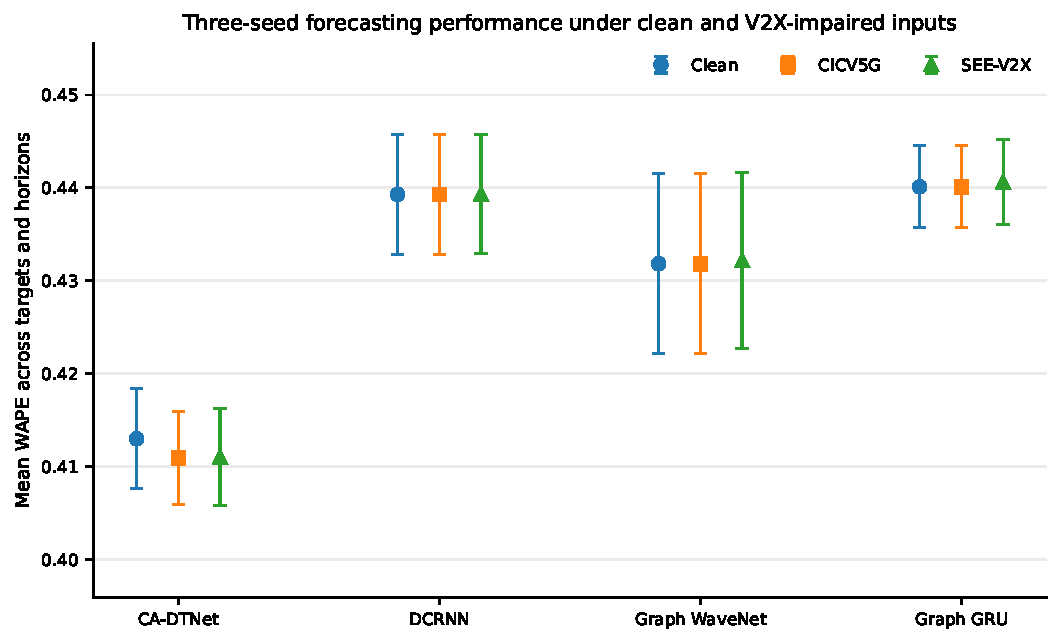
\includegraphics[width=0.98\textwidth]{Fig3_three_seed_forecasting_comparison.pdf}
    \caption{Three seed forecasting comparison across clean, CICV5G, and SEE V2X domains. The values represent WAPE aggregated across forecasting horizons and traffic targets. Lower values indicate better forecasting performance.}
    \label{fig:three_seed_forecasting}
\end{figure}

\subsection{Forecasting performance across horizon and target combinations}
\label{subsec:horizon_target_performance}

The complete evaluation includes three domains, three forecasting horizons, and three target variables. This produces twenty seven domain, horizon, and target combinations. CA-DTNet obtains the lowest MAE and WAPE in twenty four of these twenty seven combinations. Graph WaveNet obtains the lowest MAE in three specific combinations. These are thirty second vehicle count under CICV5G, ten second flow proxy under the clean domain, and thirty second vehicle count under the clean domain.

This result indicates that CA-DTNet performs strongly across most short term forecasting settings. The few cases where Graph WaveNet performs better suggest that adaptive graph convolution and dilated temporal convolution remain competitive for selected target and horizon combinations. Therefore, CA-DTNet should be interpreted as the overall strongest model in average absolute and percentage error, not as the best model for every individual metric and every individual target.

\subsection{Statistical comparison with baseline models}
\label{subsec:statistical_comparison}

To determine whether the observed improvements are consistent across paired samples, Wilcoxon signed rank tests are applied between CA-DTNet and each baseline model. Table~\ref{tab:wilcoxon_summary} summarises the number of paired comparisons in which CA-DTNet obtains lower mean error and the number of statistically significant comparisons.

\begin{table}[t]
\centering
\caption{Summary of Wilcoxon signed rank comparisons between CA-DTNet and baseline models.}
\label{tab:wilcoxon_summary}
\small
\begin{tabularx}{\linewidth}{Xccc}
\hline
Baseline & Total comparisons & CA-DTNet lower error & Significant comparisons \\
\hline
DCRNN & 81 & 75 & 66 \\
Graph WaveNet & 81 & 63 & 66 \\
Graph GRU & 81 & 77 & 74 \\
\hline
\end{tabularx}
\end{table}

The statistical results support the overall performance conclusion. CA-DTNet achieves lower error than DCRNN in seventy five of eighty one paired comparisons and is statistically significant in sixty six comparisons. Against Graph GRU, CA-DTNet obtains lower error in seventy seven of eighty one comparisons and is statistically significant in seventy four comparisons. Against Graph WaveNet, CA-DTNet obtains lower error in sixty three of eighty one comparisons and is statistically significant in sixty six comparisons.

The results show that the improvement of CA-DTNet is not limited to one domain or one forecasting horizon. At the same time, the existence of non significant cases confirms that the advantage is not uniform across all possible target and horizon combinations. This balanced result is consistent with the interpretation that CA-DTNet improves average forecasting reliability while remaining comparable to strong graph forecasting baselines.

\subsection{Digital twin reconstruction performance}
\label{subsec:reconstruction_performance}

The reconstruction head is evaluated by comparing the reconstructed traffic state with the clean traffic state. This evaluation is important because CA-DTNet is designed as a digital twin model, not only as a forecasting model. Table~\ref{tab:reconstruction_uncertainty} reports the reconstruction and probabilistic forecasting results for the full model and the objective related ablations.

\begin{table}[!htbp]
\caption{Digital twin reconstruction and probabilistic forecasting results. Reconstruction WAPE and $R^{2}$ evaluate clean-state recovery, whereas PICP and PINAW assess prediction interval coverage and sharpness, respectively.}
\label{tab:reconstruction_uncertainty}

\centering
\footnotesize
\renewcommand{\arraystretch}{1.15}
\setlength{\tabcolsep}{3pt}

\begin{tabularx}{\linewidth}{
>{\RaggedRight\arraybackslash}p{1.5cm}
>{\RaggedRight\arraybackslash}X
>{\Centering\arraybackslash}p{1.3cm}
>{\Centering\arraybackslash}p{1.3cm}
>{\Centering\arraybackslash}p{1.2cm}
>{\Centering\arraybackslash}p{1.2cm}
}

\toprule

\textbf{Domain} &
\textbf{Variant} &
\textbf{Recon. WAPE} &
\textbf{Recon. $R^{2}$} &
\textbf{PICP} &
\textbf{PINAW} \\

\midrule

CICV5G
&
Full CA-DTNet
&
0.0846
&
0.9858
&
0.7964
&
0.1180
\\

CICV5G
&
Without reconstruction loss
&
1.3181
&
$-0.2971$
&
0.7695
&
0.1235
\\

CICV5G
&
Without uncertainty loss
&
0.1009
&
0.9825
&
0.8321
&
0.2212
\\

\midrule

SEE V2X
&
Full CA-DTNet
&
0.0861
&
0.9852
&
0.7951
&
0.1181
\\

SEE V2X
&
Without reconstruction loss
&
1.3177
&
$-0.2976$
&
0.7707
&
0.1235
\\

SEE V2X
&
Without uncertainty loss
&
0.1015
&
0.9827
&
0.8322
&
0.2212
\\

\bottomrule

\multicolumn{6}{p{\dimexpr\linewidth-2\tabcolsep\relax}}{\footnotesize
\textbf{Abbreviations:}
WAPE = Weighted Absolute Percentage Error;
$R^{2}$ = Coefficient of Determination;
PICP = Prediction Interval Coverage Probability;
PINAW = Prediction Interval Normalized Average Width.
Lower WAPE and PINAW values indicate better reconstruction accuracy and sharper prediction intervals, whereas higher $R^{2}$ and PICP values indicate improved state recovery and uncertainty calibration.
}

\end{tabularx}

\end{table}

The full CA-DTNet achieves reconstruction \(R^{2}\) values of 0.9858 under CICV5G and 0.9852 under SEE V2X. These values indicate that the reconstruction head can recover the clean traffic state with high accuracy even when the input observation is communication impaired. Removing the reconstruction loss causes reconstruction performance to collapse. The reconstruction WAPE increases to approximately 1.318 in both communication domains, and the reconstruction \(R^{2}\) becomes negative. This confirms that the explicit reconstruction objective is essential for the digital twin function of the model.

Figure~\ref{fig:reconstruction} provides a visual example of the digital twin reconstruction behaviour. The reconstructed states are closely aligned with the clean states, showing that the model learns a meaningful state recovery mapping rather than only producing future forecasts.

\begin{figure}[htbp]
    \centering
    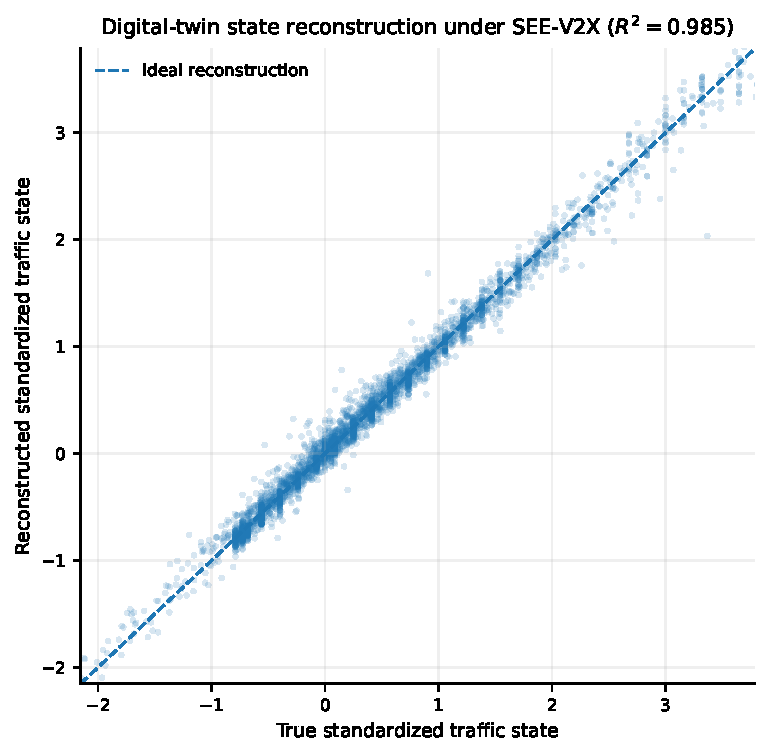
\includegraphics[width=0.90\textwidth]{Fig5_digital_twin_reconstruction.pdf}
    \caption{Digital twin reconstruction performance. The figure compares reconstructed traffic states with clean traffic states, showing the ability of CA-DTNet to recover the present physical traffic state from communication impaired observations.}
    \label{fig:reconstruction}
\end{figure}

\subsection{Probabilistic forecasting performance}
\label{subsec:probabilistic_performance}

The probabilistic forecasting head produces lower, median, and upper quantiles. The interval between the 0.10 and 0.90 quantiles is evaluated using PICP and PINAW. As shown in Table~\ref{tab:reconstruction_uncertainty}, the full model achieves PICP values of 0.7964 under CICV5G and 0.7951 under SEE V2X. The corresponding PINAW values are 0.1180 and 0.1181.

The ablation without uncertainty loss produces higher PICP values, but the interval width increases substantially. Under CICV5G, PICP increases to 0.8321, but PINAW increases to 0.2212. Under SEE V2X, PICP increases to 0.8322, while PINAW also increases to 0.2212. This means that the model without uncertainty loss achieves higher coverage mainly by producing much wider intervals. Therefore, the full model provides a better balance between coverage and sharpness.

Figure~\ref{fig:probabilistic_forecast} shows a representative probabilistic forecast. The median forecast follows the target trajectory, while the prediction interval captures uncertainty around the forecast. This behaviour is useful in communication impaired settings because the model can express reduced confidence when future traffic states are less certain.

\begin{figure}[htbp]
    \centering
    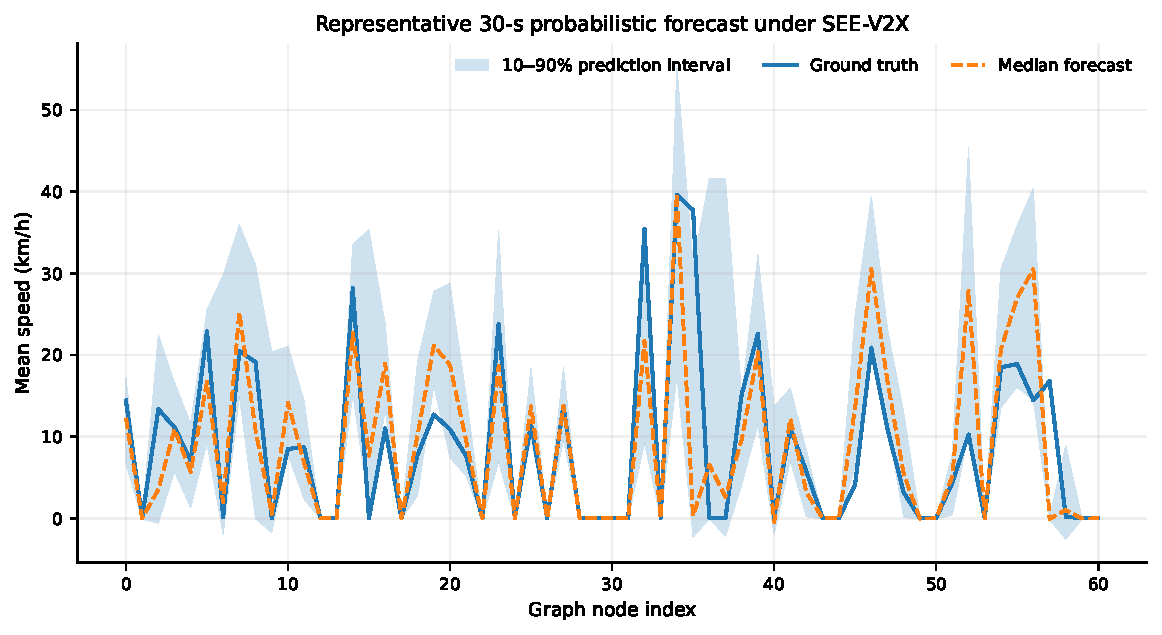
\includegraphics[width=0.90\textwidth]{Fig4_probabilistic_forecast.pdf}
    \caption{Representative probabilistic forecast generated by CA-DTNet. The median forecast is shown together with the lower and upper quantile interval. The interval represents uncertainty in the predicted traffic state.}
    \label{fig:probabilistic_forecast}
\end{figure}

\subsection{Matched communication domain robustness}
\label{subsec:matched_robustness}

A key objective of this study is to evaluate whether the model remains stable when the same physical traffic window is observed under different communication domains. For this purpose, exact matched window analysis is performed between CICV5G and SEE V2X observations. Each comparison uses the same underlying traffic window and changes only the communication trace.

Table~\ref{tab:matched_domain_robustness} reports the number of horizon and target tasks with statistically significant communication domain effects. CA-DTNet shows a significant communication domain effect in one of nine tasks. Graph GRU shows significant effects in five of nine tasks. Persistence shows significant effects in two of nine tasks, while Impaired GRU shows significant effects in one of nine tasks.

\begin{table}[t]
\centering
\caption{Matched communication domain robustness under exact paired traffic windows. Lower significant fraction indicates higher communication domain stability.}
\label{tab:matched_domain_robustness}
\small
\begin{tabular}{p{3.5cm} p{3.0cm} p{3.2cm}}
\hline
Model & Significant tasks & Significant fraction \\
\hline
CA-DTNet & 1 of 9 & 11.1 percent \\
Impaired GRU & 1 of 9 & 11.1 percent \\
Persistence & 2 of 9 & 22.2 percent \\
Graph GRU & 5 of 9 & 55.6 percent \\
\hline
\end{tabular}
\end{table}

The matched analysis supports the communication robustness claim of CA-DTNet. Since the physical traffic window is fixed, differences between CICV5G and SEE V2X can be attributed to communication domain variation rather than traffic difficulty. The low fraction of significant domain effects indicates that CA-DTNet is comparatively stable across heterogeneous communication traces.

Figure~\ref{fig:matched_domain_robustness} visualises the matched domain robustness results. The lower fraction for CA-DTNet indicates that its errors are less sensitive to the change from CICV5G to SEE V2X than those of Graph GRU.

\begin{figure}[htbp]
    \centering
    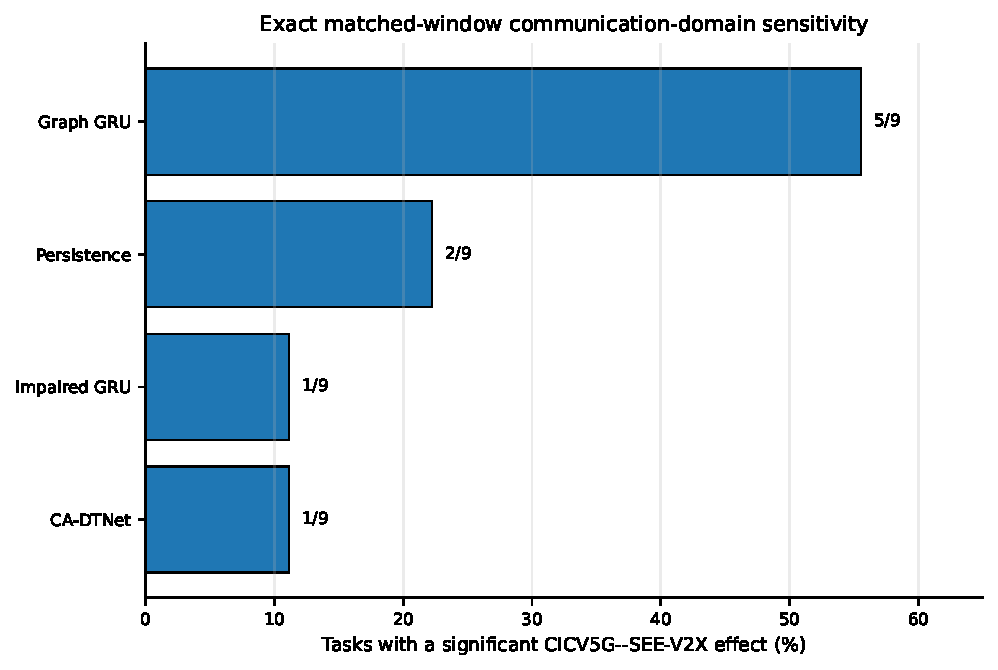
\includegraphics[width=0.90\textwidth]{Fig6_matched_domain_robustness.pdf}
    \caption{Matched communication domain robustness. The figure reports the fraction of horizon and target tasks for which the error difference between CICV5G and SEE V2X is statistically significant under matched traffic windows. Lower values indicate stronger communication domain stability.}
    \label{fig:matched_domain_robustness}
\end{figure}

\begin{changed}
Across the nine matched CA-DTNet tasks, the absolute CICV5G-to-SEE-V2X MAE shift averages 0.20\% and never exceeds 0.81\%. The only significant task is 30-s vehicle count (CICV5G MAE 1.5860, SEE-V2X MAE 1.5732, relative shift $-0.80$\%, Wilcoxon \(p=2.21\times10^{-5}\)). Statistical significance here reflects the consistency of a small paired shift across 74 windows, not a large operational degradation. These held-out windows expose unseen temporal trace segments, but both communication domain identities were present during training. The result therefore quantifies sensitivity to heterogeneous held-out conditions; it is not evidence of zero-shot generalization to a third radio domain.
\end{changed}

\subsection{Component ablation study}
\label{subsec:ablation_results}

The component ablation study evaluates the contribution of communication encoding, age of information, graph attention, reconstruction supervision, and uncertainty learning. Table~\ref{tab:ablation_point_forecasting} reports the point forecasting ablation results. The complete CA-DTNet is compared with variants that remove one component at a time.

\begin{table}[!htbp]
\caption{Component ablation for point forecasting. WAPE and $R^{2}$ are averaged over the three horizons and three targets. Negative $\Delta$WAPE means that removing the component reduced point error.}
\label{tab:ablation_point_forecasting}
\centering
\footnotesize
\renewcommand{\arraystretch}{1.15}
\setlength{\tabcolsep}{2.5pt}
\begin{tabular}{lrrrrrr}
\toprule
\multirow{2}{*}{Variant} & \multicolumn{3}{c}{CICV5G} & \multicolumn{3}{c}{SEE-V2X} \\
\cmidrule(lr){2-4}\cmidrule(lr){5-7}
& WAPE & $\Delta$ (\%) & $R^2$ & WAPE & $\Delta$ (\%) & $R^2$ \\
\midrule
Full CA-DTNet & 0.4160 & 0.00 & 0.6659 & 0.4154 & 0.00 & 0.6672 \\
Without communication encoder & 0.4073 & $-2.10$ & 0.6772 & 0.4074 & $-1.92$ & 0.6772 \\
Without AoI & 0.4038 & $-2.94$ & 0.6775 & 0.4037 & $-2.80$ & 0.6769 \\
Without graph attention & 0.4230 & 1.67 & 0.6447 & 0.4224 & 1.70 & 0.6458 \\
Without reconstruction loss & 0.4102 & $-1.39$ & 0.6643 & 0.4087 & $-1.61$ & 0.6668 \\
Without uncertainty loss & 0.4126 & $-0.83$ & 0.6929 & 0.4113 & $-0.98$ & 0.6952 \\
\bottomrule
\end{tabular}
\end{table}

The ablation results require careful interpretation. Removing graph attention increases WAPE in both communication domains. This confirms that spatial graph learning contributes positively to point forecasting performance. However, removing the communication encoder or age of information slightly reduces WAPE in this specific point forecasting evaluation. This does not mean that communication awareness is unnecessary. Communication variables also support domain awareness, reconstruction, uncertainty modelling, and matched robustness, which are not fully captured by point WAPE alone.

The reconstruction and uncertainty ablations further clarify this point. Removing reconstruction loss causes a major collapse in digital twin state recovery, as shown in Table~\ref{tab:reconstruction_uncertainty}. Removing uncertainty loss increases interval width substantially. Therefore, the proposed model components should be evaluated according to their corresponding roles. Graph attention supports point forecasting. Reconstruction supervision supports clean state recovery. Uncertainty learning supports sharper probabilistic intervals. Communication features support the broader objective of communication aware digital twin operation.

\begin{changed}
The loss-weight evidence is an endpoint sensitivity analysis rather than a dense hyperparameter sweep. At the reported \(\lambda_r=0.3\), reconstruction WAPE is 0.0846/0.0861 and reconstruction \(R^2\) is 0.9858/0.9852 for CICV5G/SEE-V2X. Setting \(\lambda_r=0\) increases reconstruction WAPE to 1.3181/1.3177 and makes \(R^2\) negative, while point WAPE changes from 0.4160/0.4154 to 0.4102/0.4087. Thus reconstruction supervision substantially improves state fidelity but entails a 1.39--1.61\% point-WAPE trade-off. This is precisely why the auxiliary weight is kept below the forecasting weight and why the paper does not claim that reconstruction supervision improves every forecasting metric. A denser \(\lambda_r\) sweep would require retraining and remains part of the stated sensitivity limitation.
\end{changed}

\subsection{Communication trace characteristics}
\label{subsec:communication_trace_characteristics}

The communication trace characteristics are visualised in Fig.~\ref{fig:communication_trace_characteristics}. The figure compares the normalized behaviour of the communication variables in CICV5G and SEE V2X. The two communication domains show different profiles, which justifies the need for domain aware evaluation. If both communication traces behaved similarly, then matched robustness analysis would provide limited additional insight. The observed difference between the domains makes it necessary to test whether forecasting performance remains stable when the same traffic window is observed under different communication conditions.

\begin{figure}[htbp]
    \centering
    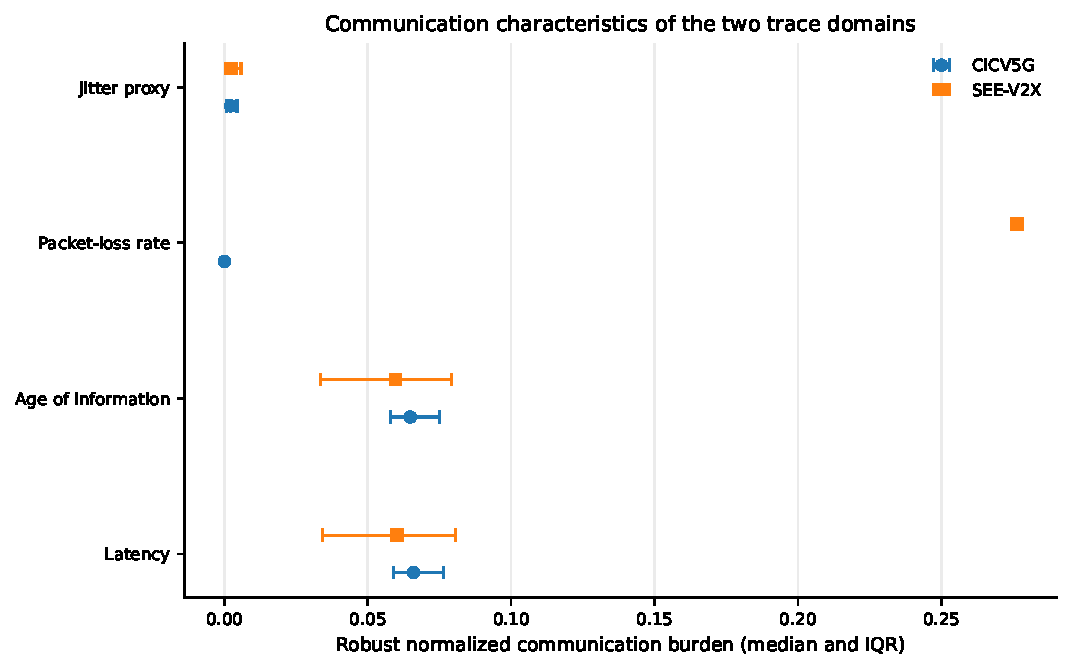
\includegraphics[width=0.90\textwidth]{Fig2_communication_trace_characteristics.pdf}
    \caption{Communication trace characteristics for CICV5G and SEE V2X. The figure summarises normalized communication burden across representative communication variables. The difference between the two domains motivates the communication aware and matched robustness evaluation.}
    \label{fig:communication_trace_characteristics}
\end{figure}

\subsection{Computational efficiency}
\label{subsec:efficiency_results}

Computational efficiency is important for traffic digital twin deployment because the model should operate close to real time. Table~\ref{tab:efficiency_results} reports parameter count, checkpoint size, training time, inference latency, and peak GPU memory for the learned models.

\begin{table*}[t]
\centering
\caption{Computational efficiency comparison. Inference latency is reported per sample.}
\label{tab:efficiency_results}
\small
\begin{adjustbox}{max width=\textwidth}
\begin{tabular}{lrrrrr}
\hline
Model & Parameters & Checkpoint size & Training time & Latency per sample & Peak GPU memory \\
\hline
DCRNN & 124233 & 0.5370 MB & 339.3957 s & 7.4015 ms & 53.4360 MB \\
Graph WaveNet & 98541 & 0.4274 MB & 117.4943 s & 1.1185 ms & 198.7012 MB \\
Graph GRU & 34377 & 0.1506 MB & 31.7186 s & 0.1676 ms & 328.4126 MB \\
CA-DTNet & 71203 & 0.2888 MB & 102.8372 s & 0.3933 ms & 385.6001 MB \\
\hline
\end{tabular}
\end{adjustbox}
\end{table*}

CA-DTNet contains 71,203 trainable parameters and has a checkpoint size of 0.2888 MB. Its inference latency is approximately 0.3933 ms per sample. Graph GRU is faster, with 0.1676 ms per sample, but it does not provide the same combination of communication aware encoding, digital twin reconstruction, and probabilistic forecasting. DCRNN is substantially slower, requiring 7.4015 ms per sample. Graph WaveNet requires 1.1185 ms per sample. Therefore, CA-DTNet provides a practical compromise between functionality and inference efficiency.

Figure~\ref{fig:efficiency_accuracy} presents the accuracy and efficiency tradeoff. CA-DTNet achieves the lowest overall WAPE while maintaining low inference latency and moderate parameter count.

\begin{figure}[htbp]
    \centering
    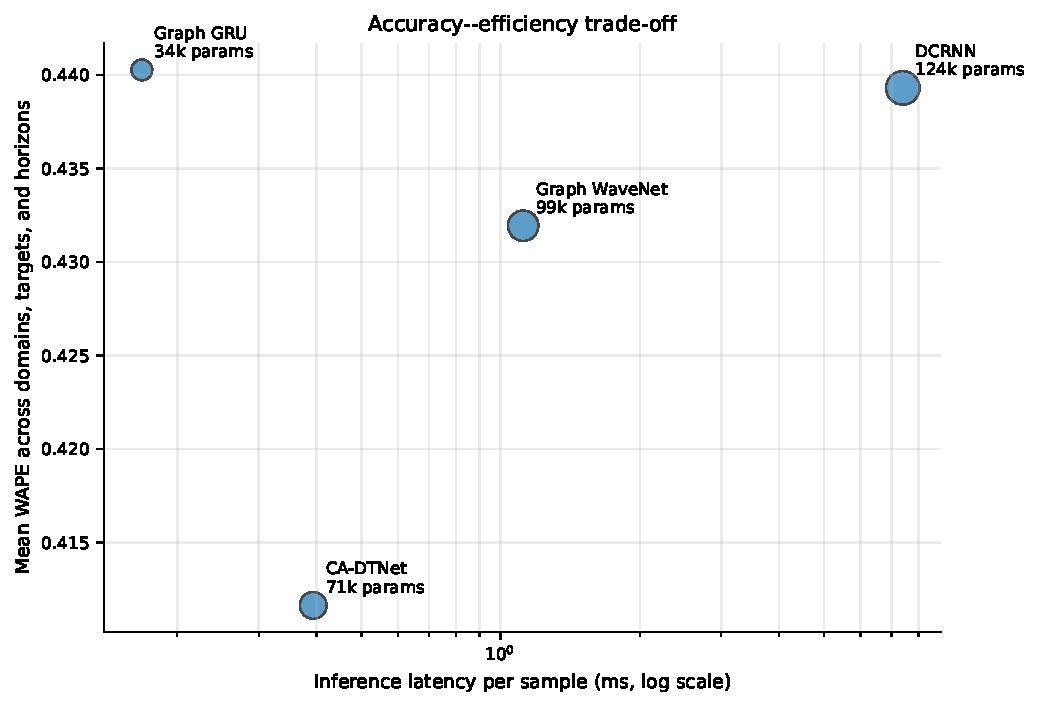
\includegraphics[width=0.90\textwidth]{Fig7_efficiency_accuracy_tradeoff.pdf}
    \caption{Accuracy and efficiency tradeoff. The horizontal axis represents inference latency per sample, and the vertical axis represents overall WAPE. CA-DTNet achieves low WAPE with practical inference latency and moderate model size.}
    \label{fig:efficiency_accuracy}
\end{figure}

\subsection{Summary of findings}
\label{subsec:results_summary}

The experimental results support five main findings. First, CA-DTNet achieves the lowest WAPE across clean, CICV5G, and SEE V2X domains. Second, it obtains the best MAE and WAPE in twenty four of twenty seven domain, horizon, and target combinations. Third, the reconstruction head successfully recovers the clean digital twin state, with reconstruction \(R^{2}\) above 0.985 in both communication domains. Fourth, the probabilistic forecasting head provides a balanced interval with approximately 0.795 coverage and 0.118 normalized interval width. Fifth, the matched domain analysis shows that CA-DTNet is stable across heterogeneous communication traces, with a significant communication domain effect in only one of nine forecasting tasks.

These findings confirm that CA-DTNet should be interpreted as a communication aware digital twin framework rather than only as a point forecasting model. Its main advantage is the joint ability to forecast traffic, reconstruct the clean present state, represent uncertainty, and maintain stability under different measured vehicular communication conditions.

\section{Discussion}
\label{sec:discussion}

The results in Section~\ref{sec:results} show that CA-DTNet provides a reliable communication aware digital twin framework for high resolution traffic forecasting. This section discusses the meaning of the obtained results, explains the role of each major model component, analyses the communication robustness behaviour, and clarifies the practical implications and limitations of the study.

\subsection{Interpretation of forecasting performance}
\label{subsec:discussion_forecasting}

The overall forecasting results show that CA-DTNet achieves the lowest WAPE in the clean, CICV5G, and SEE V2X domains. This indicates that the proposed model reduces average percentage based forecasting error under both clean and communication impaired conditions. The improvement is consistent across the three evaluation domains, which suggests that the model does not rely on a single communication setting or a single observation condition.

The result is important because traffic forecasting in connected vehicular environments cannot be evaluated only under clean observations. In practice, traffic data may be delayed, stale, or incomplete before reaching the digital platform. A model that performs well only under clean observations may not be reliable when deployed in a communication dependent system. CA-DTNet addresses this issue by learning from traffic and communication histories together. The traffic encoder captures mobility dynamics, while the communication encoder provides contextual information about the reliability and freshness of the received observations.

The model obtains the best MAE and WAPE in twenty four of twenty seven evaluated domain, horizon, and target combinations. This shows that the performance gain is not isolated to a single horizon or target. However, Graph WaveNet remains better in three individual MAE cases. This confirms that CA-DTNet should not be described as universally superior on every metric. Its main strength is the combination of low average absolute error, low percentage error, domain stability, state reconstruction, uncertainty estimation, and computational feasibility.

The \(R^{2}\) results also require careful interpretation. DCRNN achieves higher overall \(R^{2}\) values than CA-DTNet. This means that DCRNN remains competitive in squared error based evaluation. Since \(R^{2}\) is strongly influenced by large deviations, this result suggests that CA-DTNet is more effective in reducing average absolute and percentage based error, while DCRNN can still explain a larger portion of variance in some settings. Therefore, the contribution of CA-DTNet is not based on claiming dominance across all numerical measures. Instead, the contribution lies in providing a broader and more deployment oriented modelling framework.

\subsection{Role of communication awareness}
\label{subsec:discussion_communication_awareness}

A central question in this study is whether communication context improves traffic forecasting. The answer is not a simple yes for every point metric. The ablation study shows that removing the communication encoder or age of information slightly reduces WAPE in the point forecasting ablation table. This observation is important and should not be ignored. It indicates that communication variables do not automatically improve every point forecasting metric when they are added to a neural network.

However, this does not invalidate the role of communication awareness. The goal of CA-DTNet is not only to minimise point forecasting error. The goal is to construct a communication aware digital twin that can operate under heterogeneous vehicular communication conditions. Communication context contributes to this broader objective in several ways. It provides information about observation freshness, helps interpret whether a traffic state may be delayed or unreliable, supports matched communication domain evaluation, and enables the model to connect forecasting behaviour with measured network conditions.

The matched-domain analysis provides additional evidence for this interpretation. Across the nine CA-DTNet horizon--target tasks, the absolute CICV5G-to-SEE-V2X MAE shift averages 0.20\% and does not exceed 0.81\%. Only the 30-s vehicle-count task is statistically significant, whereas Graph GRU has significant effects in five of nine tasks. Because each pair uses the same 74 physical traffic windows, the comparison removes traffic-window difficulty as a confounder. The small but consistent 30-s shift also illustrates why statistical significance must be interpreted together with effect magnitude.

Therefore, communication awareness should be interpreted as a robustness and digital twin capability rather than only as a mechanism for reducing point WAPE in every ablation setting. This interpretation is consistent with the research objective of the manuscript.

\subsection{Importance of digital twin reconstruction}
\label{subsec:discussion_reconstruction}

The reconstruction results strongly support the digital twin component of CA-DTNet. The full model achieves reconstruction \(R^{2}\) above 0.985 in both CICV5G and SEE V2X domains. This means that the model can recover the clean present traffic state from communication impaired observations with high accuracy.

The reconstruction ablation further confirms the importance of this component. When the reconstruction loss is removed, reconstruction WAPE increases sharply and reconstruction \(R^{2}\) becomes negative. This indicates that accurate digital twin state recovery does not emerge automatically from the forecasting objective. It must be explicitly encouraged during training.

This finding has practical relevance. A traffic digital twin is expected to maintain an accurate virtual representation of the physical road state. If the model only predicts future traffic but fails to reconstruct the present state, it cannot fully support digital twin operation. The reconstruction head therefore provides an additional layer of functionality beyond conventional forecasting. It enables the model to estimate the current clean traffic condition even when the received observation is affected by communication impairment.

\subsection{Uncertainty estimation and interval quality}
\label{subsec:discussion_uncertainty}

The probabilistic forecasting results show that CA-DTNet provides prediction intervals with balanced coverage and sharpness. The full model achieves PICP values close to 0.795 in both communication domains with PINAW values close to 0.118. This indicates that the prediction intervals cover a substantial portion of the true values while remaining relatively narrow.

The uncertainty ablation provides a useful comparison. When the uncertainty loss is removed, PICP increases, but PINAW also increases substantially. This means that higher coverage is achieved mainly by producing wider intervals. A wider interval is not always better because it may become less useful for traffic management decisions. In practical systems, a forecast interval should be reliable but not unnecessarily broad.

The full CA-DTNet therefore provides a more balanced probabilistic output. This is important in communication impaired traffic forecasting because uncertainty may increase when observations are delayed, stale, or incomplete. A digital twin should be able to express such uncertainty rather than producing only a single deterministic forecast.

\subsection{Role of graph attention}
\label{subsec:discussion_graph_attention}

The ablation study shows that removing graph attention increases WAPE in both communication domains. This result confirms the importance of spatial graph learning in the proposed architecture. Traffic states at neighbouring or functionally related road segments are dependent. Congestion, queue formation, and speed reduction can propagate across the network. A node independent model would ignore these spatial dependencies.

Graph attention is especially suitable for the proposed framework because the influence of neighbouring nodes may vary across time and communication conditions. A fixed spatial aggregation may not always capture this variation. The attention mechanism allows the model to assign different importance to neighbouring nodes based on the learned fused representation. Since the fused representation already contains traffic and communication information, the spatial encoder can learn graph interactions under the current observation context.

This explains why the graph attention component contributes positively to point forecasting performance. It helps the model represent network wide traffic interactions while remaining adaptive to the learned traffic communication state.

\subsection{Communication domain robustness}
\label{subsec:discussion_domain_robustness}

The matched communication domain analysis is one of the most important parts of the study. Conventional evaluation compares models across test domains, but such comparisons may be confounded by traffic difficulty. A model may appear worse under one communication domain simply because that domain is associated with more difficult traffic windows. The matched analysis avoids this problem by comparing CICV5G and SEE V2X observations generated from the same physical traffic window.

The results show that CA-DTNet has a low fraction of significant communication-domain effects and small paired effect magnitudes. Its prediction error remains comparatively stable when the replay domain changes while the traffic state remains the same. Because both domain identities occur in training, this finding supports robustness to held-out trace segments from the two studied domains; it does not establish zero-shot transfer to a third radio domain.

This does not mean that communication has no effect on prediction. Communication quality can still affect the received traffic observation. The result means that CA-DTNet is better able to absorb or compensate for such variation than some baseline models. This behaviour is desirable for real vehicular digital twins because the communication environment can change across network technologies, channel conditions, and deployment regions.

\subsection{Efficiency and deployability}
\label{subsec:discussion_efficiency}

Efficiency analysis shows that CA-DTNet has a moderate number of parameters and low inference latency. The model uses 71,203 trainable parameters and requires approximately 0.3933 milliseconds per sample. This latency is higher than Graph GRU but much lower than DCRNN and Graph WaveNet. Graph GRU is the fastest model, but it does not provide the same set of functions as CA-DTNet. It does not include explicit communication aware fusion, digital twin reconstruction, and probabilistic forecasting in the same framework.

Therefore, CA-DTNet provides a practical tradeoff. It is not the smallest or fastest model, but it offers a richer set of capabilities while remaining computationally lightweight. This is important for near real time traffic digital twin applications, where inference speed, model size, and functional capability must be considered together.

\subsection{Practical implications}
\label{subsec:discussion_practical_implications}

The proposed framework has several practical implications for intelligent transportation systems. First, it suggests that traffic forecasting models should consider communication conditions when the data are transmitted through vehicular networks. The quality of the received observation depends not only on the physical traffic state but also on the communication process.

Second, the reconstruction head provides a mechanism for maintaining a clean digital twin state. This can be useful for traffic monitoring platforms where the received data stream is affected by delay or missing updates. Instead of directly using the impaired observation, the system can use the reconstructed state as a more reliable estimate of the current traffic condition.

Third, the probabilistic output can support risk aware decision making. Traffic control and routing decisions can be more reliable when the system knows not only the predicted value but also the uncertainty around that prediction. This is especially relevant when communication conditions are poor.

Fourth, the matched communication domain evaluation provides a useful experimental strategy for future studies. By holding the traffic window fixed and changing only the communication trace, researchers can better isolate the effect of communication variation on forecasting performance.

\subsection{Limitations}
\label{subsec:discussion_limitations}

\begin{changed}
The evidence is bounded by one traffic source, one city, and two communication datasets. pNEUMA was selected because its naturalistic trajectories support one-second, graph-structured states; CICV5G and SEE-V2X were selected because their complementary cellular and sidelink measurements contain the delay, loss, AoI-related, load, throughput, and radio-quality variables required by the replay. This combination supports a controlled proof of concept, but it cannot establish geographic transfer beyond Athens or network transfer to unobserved technologies, densities, or propagation environments.

The traffic and communication datasets have neither a common clock nor common coordinates. The index-aligned replay preserves the ordering and within-trace co-variation of measured communication samples, but it does not claim geographic co-location. Cycling trace identifiers across road nodes and using seeded contiguous offsets prevents outcome-based pairing, yet repeated assignment can underrepresent correlations that would arise when many nearby vehicles share the same channel. Future work should collect synchronized traffic--radio measurements or validate the framework with calibrated microscopic traffic and network co-simulation.

Both CICV5G and SEE-V2X appear in training. The held-out test split contains unseen chronological traffic windows and unseen trace segments, not a wholly unseen communication domain. The matched-domain experiment therefore measures sensitivity within the supported domain set rather than zero-shot domain generalization. Evaluation on another city and a third, strictly held-out communication dataset is required before claiming cross-geographic or cross-technology transfer.

The loss-weight study compares the selected \(\lambda_r=0.3\) with the no-reconstruction endpoint \(\lambda_r=0\); it is not a dense sensitivity sweep. The endpoint analysis exposes the trade-off clearly---large reconstruction gains with a 1.39--1.61\% point-WAPE cost---but retraining a broader coefficient grid would better characterize the Pareto frontier. Similarly, recent Transformer models are discussed but are not included as numerical baselines because the available published results use different datasets, resolutions, targets, and inputs. A future benchmark should reimplement these models under the same replay protocol.

Finally, CA-DTNet does not dominate every metric. DCRNN has higher overall \(R^{2}\), Graph WaveNet is better in a small number of individual MAE cases, and removal of communication variables can slightly improve point WAPE. The communication branch is therefore justified by state interpretation and domain-aware robustness rather than universal point-error reduction. The current study also stops at forecasting and reconstruction; downstream effects on signal control, routing, or cooperative driving remain to be measured.
\end{changed}

\subsection{Future research directions}
\label{subsec:discussion_future_work}

Several future directions can extend the present work. First, the framework can be evaluated on additional urban networks and traffic datasets to test transferability across locations. Second, more communication domains can be included, such as different NR V2X configurations, edge assisted communication traces, or mixed communication environments. Third, the communication aware fusion mechanism can be improved using attention based reliability weighting or uncertainty guided gating. Fourth, conformal calibration can be integrated with the quantile forecasts to improve coverage guarantees under distribution shift. Fifth, the reconstructed digital twin state can be connected with traffic control or route guidance modules to evaluate decision level benefits.

These directions would further strengthen the connection between traffic forecasting, vehicular communication, digital twin state estimation, and intelligent transportation decision support.

\section{Conclusion}
\label{sec:conclusion}

\begin{changed}
This paper presented CA-DTNet, a trace-driven, communication-aware digital twin for high-resolution traffic forecasting. The replay maps ordered communication samples to one-second traffic bins with fixed, seeded assignments. Loss events generate sample-and-hold observations and increasing AoI, while the remaining measured network variables condition a reliability gate. A shared 64-dimensional spatiotemporal representation supports clean-state reconstruction and quantile forecasts at 5-, 10-, and 30-s horizons.

Under the common protocol, CA-DTNet records the lowest mean MAE and WAPE in 24 of 27 domain--horizon--target combinations. Reconstruction \(R^{2}\) exceeds 0.985 in both communication domains. The matched-window analysis gives a mean absolute CICV5G-to-SEE-V2X MAE shift of 0.20\%, a maximum of 0.81\%, and one significant task out of nine. The model uses 71,203 parameters---fewer than DCRNN and Graph WaveNet---and requires approximately 0.393~ms per sample, so the reported gains are not attributable to greater parameter count alone.

The ablations also qualify the interpretation. Graph attention improves point forecasting, reconstruction supervision is necessary for accurate state recovery, and probabilistic training yields substantially sharper intervals. Communication encoding and AoI do not improve every point-WAPE value; their role is chiefly to make the observation process explicit and to support stable, interpretable operation across the two measured domains. The current evidence remains limited to pNEUMA and two communication datasets whose clocks and locations are not co-registered. Validation on another city and a strictly unseen radio domain is therefore the principal next step. Within these boundaries, CA-DTNet connects traffic prediction, measured communication impairment, present-state reconstruction, and calibrated uncertainty in one reproducible framework.
\end{changed}

\section*{Reproducibility Statement}

To support independent verification, we provide the complete CA-DTNet
implementation, training scripts, released model checkpoints, prediction
arrays, statistical analyses, manuscript figures, and result tables in a
version-controlled reproducibility repository at
\url{https://github.com/shishirbit/CADTNet}. The repository is private during
peer review and will be made publicly accessible upon publication. The
submitted source package and repository manifest identify the exact files used
for this study.

The experiments use chronological data partitions comprising 70\% training,
15\% validation, and 15\% testing samples. All reported models were evaluated
with random seeds 42, 52, and 62 using identical input histories, forecast
horizons, target variables, and evaluation metrics. Data normalization
parameters were estimated exclusively from the training partition to prevent
future-information leakage.

The released prediction arrays allow the reported MAE, RMSE, WAPE, and
coefficient-of-determination ($R^2$) values to be recomputed independently
without retraining the models. Running
\texttt{python scripts/verify\_results.py} recomputes 108 seed-42 metric rows,
verifies 432 three-seed aggregate values, and confirms that CA-DTNet obtains
the lowest mean MAE and WAPE in 24 of the 27 evaluated
domain--horizon--target configurations.

Raw pNEUMA, CICV5G, and SEE-V2X datasets are not redistributed because of
their size and original access conditions. The repository instead provides a
dataset-acquisition script, records the official data sources, and implements
the complete trajectory-processing, communication-trace standardization, and
trace-replay procedures. SHA-256 checksums are included for the released
checkpoints and result artifacts. Because execution time depends on hardware
and software configuration, timing results should be compared only under the
same computational environment.


\section*{Declarations}
\label{sec:declarations}

\subsection*{Funding}

The authors did not receive any specific grant from funding agencies in the public, commercial, or not for profit sectors for this work.

\subsection*{Conflict of interest}

The authors declare that they have no known competing financial interests or personal relationships that could have appeared to influence the work reported in this paper.

\subsection*{Ethical approval}

This study does not involve human participants, human biological material, or animal experiments. The experiments are conducted using publicly available traffic trajectory data and communication trace data.

\subsection*{Informed consent}

Not applicable.

\subsection*{Author contributions}

\textbf{Shishir Singh Chauhan} conceived the research idea, formulated the problem statement, designed the CA DTNet framework, and developed the overall methodology of the study. He performed the literature review, prepared the communication aware digital twin formulation, designed the trace driven evaluation protocol, and carried out the preprocessing of pNEUMA traffic trajectories with CICV5G and SEE V2X communication traces. He implemented the proposed CA DTNet model, baseline models, and ablation variants. He conducted the forecasting experiments, digital twin reconstruction analysis, probabilistic forecasting evaluation, matched communication domain robustness analysis, statistical testing, and computational efficiency assessment. He analysed and interpreted the experimental results, prepared the figures and tables, and wrote the initial draft of the manuscript.\\\\
\textbf{Satyabrata Roy} supervised the research work and contributed to the refinement of the problem formulation, methodology, experimental design, and result interpretation. He critically reviewed the proposed framework, provided intellectual input for positioning the work within intelligent transportation systems and communication-aware digital twin research, and guided the organisation of the manuscript. He also reviewed the results, checked the technical consistency of the manuscript, and provided critical editorial guidance to improve the clarity, scientific quality, and overall presentation of the paper.\\\\
Both authors reviewed and approved the final version of the manuscript.

\subsection*{Data availability}

The pNEUMA trajectory dataset used for traffic state construction is publicly available from the original pNEUMA open traffic data source at \url{https://open-traffic.epfl.ch/}. The communication traces used in this study are processed for trace-driven replay and evaluation. The processed traffic states, aligned communication inputs, trained model outputs, and result files are documented in the private review repository and can also be provided by the corresponding author subject to the source datasets' access conditions.

\subsection*{Code availability}

The implementation code used for preprocessing, model training, evaluation, ablation, matched robustness analysis, and figure generation is available in the private review repository at \url{https://github.com/shishirbit/CADTNet}; it will be released publicly upon publication.

\subsection*{Acknowledgements}

The authors would like to acknowledge the availability of high resolution traffic trajectory data and vehicular communication traces that made this trace driven study possible.

\bibliography{sn-bibliography}% common bib file
%% if required, the content of .bbl file can be included here once bbl is generated
%%\input sn-article.bbl

\end{document}
